%%%%%%%%%%%%%%%%%%%%%%%%%%%%%%%%%%%%%%%%%%%%%%%%%%%%%%%%%%%%%%%%%%%%%%%
%
%  A small sample UNSW Coursework Masters thesis file.
%  Any questions to Ian Doust i.doust@unsw.edu.au and/or Gery Geenens ggeenens@unsw.edu.au
%
%%%%%%%%%%%%%%%%%%%%%%%%%%%%%%%%%%%%%%%%%%%%%%%%%%%%%%%%%%%%%%%%%%%%%%%
%
%  The first part pulls in a UNSW Thesis class file.  This one is
%  slightly nonstandard and has been set up to do a couple of
%  things automatically
%
 
%%%%%%%%%%%%%%%%%
%% Precisely one of the next four lines should be uncommented.
%% Choose the one which matches your degree, uncomment it, and comment out the other two!
%\documentclass[mfin,12pt]{unswthesis}    %%  For Master of Financial Mathematics 
%\documentclass[mmath,12pt]{unswthesis}   %%  For Master of Mathematics
\documentclass[mstat,12pt]{unswthesis}  %%  For Master of Statistics
%%%%%%%%%%%%%%%%%


\linespread{1}
\usepackage{amsfonts}
\usepackage{float}
\usepackage{amssymb}
\usepackage{amsthm}
\usepackage{latexsym,amsmath}
\usepackage{graphicx}
\usepackage{afterpage}
\usepackage[ruled,vlined]{algorithm2e}
\usepackage{dsfont}
\usepackage{caption}
\usepackage{subcaption}
\usepackage{hyperref}
\usepackage{listings}
\usepackage{float}

%%%%%%%%%%%%%%%%%%%%%%%%%%%%%%%%%%%%%%%%%%%%%%%%%%%%%%%%%%%%%%%%%
%
%  The following are some simple LaTeX macros to give some
%  commonly used letters in funny fonts. You may need more or less of
%  these
%
\newcommand{\R}{\mathbb{R}}
\newcommand{\Q}{\mathbb{Q}}
\newcommand{\C}{\mathbb{C}}
\newcommand{\N}{\mathbb{N}}
\newcommand{\F}{\mathbb{F}}
\newcommand{\PP}{\mathbb{P}}
\newcommand{\T}{\mathbb{T}}
\newcommand{\Z}{\mathbb{Z}}
\newcommand{\B}{\mathfrak{B}}
\newcommand{\BB}{\mathcal{B}}
\newcommand{\M}{\mathfrak{M}}
\newcommand{\X}{\mathfrak{X}}
\newcommand{\Y}{\mathfrak{Y}}
\newcommand{\CC}{\mathcal{C}}
\newcommand{\E}{\mathbb{E}}
\newcommand{\cP}{\mathcal{P}}
\newcommand{\cS}{\mathcal{S}}
\newcommand{\A}{\mathcal{A}}
\newcommand{\ZZ}{\mathcal{Z}}
%%%%%%%%%%%%%%%%%%%%%%%%%%%%%%%%%%%%%%%%%%%%%%%%%%%%%%%%%%%%%%%%%%%%%
%
% The following are much more esoteric commands that I have left in
% so that this file still processes. Use or delete as you see fit
%
\newcommand{\bv}[1]{\mbox{BV($#1$)}}
\newcommand{\comb}[2]{\left(\!\!\!\begin{array}{c}#1\\#2\end{array}\!\!\!\right)
}
\newcommand{\Lat}{{\rm Lat}}
\newcommand{\var}{\mathop{\rm var}}
\newcommand{\Pt}{{\mathcal P}}
\def\tr(#1){{\rm trace}(#1)}
\def\Exp(#1){{\mathbb E}(#1)}
\def\Exps(#1){{\mathbb E}\sparen(#1)}
\newcommand{\floor}[1]{\left\lfloor #1 \right\rfloor}
\newcommand{\ceil}[1]{\left\lceil #1 \right\rceil}
\newcommand{\hatt}[1]{\widehat #1}
\newcommand{\modeq}[3]{#1 \equiv #2 \,(\text{mod}\, #3)}
\newcommand{\rmod}{\,\mathrm{mod}\,}
\newcommand{\p}{\hphantom{+}}
\newcommand{\vect}[1]{\mbox{\boldmath $ #1 $}}
\newcommand{\reff}[2]{\ref{#1}.\ref{#2}}
\newcommand{\psum}[2]{\sum_{#1}^{#2}\!\!\!'\,\,}
\newcommand{\bin}[2]{\left( \begin{array}{@{}c@{}}
				#1 \\ #2
			\end{array}\right)	}
%
%  Macros - some of these are in plain TeX (gasp!)
%
\newcommand{\be}{($\beta$)}
\newcommand{\eqp}{\mathrel{{=}_p}}
\newcommand{\ltp}{\mathrel{{\prec}_p}}
\newcommand{\lep}{\mathrel{{\preceq}_p}}
\def\brack#1{\left \{ #1 \right \}}
\def\bul{$\bullet$\ }
\def\cl{{\rm cl}}
\let\del=\partial
\def\enditem{\par\smallskip\noindent}
\def\implies{\Rightarrow}
\def\inpr#1,#2{\t \hbox{\langle #1 , #2 \rangle} \t}
\def\ip<#1,#2>{\langle #1,#2 \rangle}
\def\lp{\ell^p}
\def\maxb#1{\max \brack{#1}}
\def\minb#1{\min \brack{#1}}
\def\mod#1{\left \vert #1 \right \vert}
\def\norm#1{\left \Vert #1 \right \Vert}
\def\paren(#1){\left( #1 \right)}
\def\qed{\hfill \hbox{$\Box$} \smallskip}
\def\sbrack#1{\Bigl \{ #1 \Bigr \} }
\def\ssbrack#1{ \{ #1 \} }
\def\smod#1{\Bigl \vert #1 \Bigr \vert}
\def\smmod#1{\bigl \vert #1 \bigr \vert}
\def\ssmod#1{\vert #1 \vert}
\def\sspmod#1{\vert\, #1 \, \vert}
\def\snorm#1{\Bigl \Vert #1 \Bigr \Vert}
\def\ssnorm#1{\Vert #1 \Vert}
\def\sparen(#1){\Bigl ( #1 \Bigr )}

\newcommand\blankpage{%
    \null
    \thispagestyle{empty}%
    \addtocounter{page}{-1}%
    \newpage}

%%%%%%%%%%%%%%%%%%%%%%%%%%%%%%%
%
% These environments allow you to get nice numbered headings
%  for your Theorems, Definitions etc.  
%
%  Environments
%
%%%%%%%%%%%%%%%%%%%%%%%%%%%%%%%

\newtheorem{theorem}{Theorem}[section]
\newtheorem{lemma}[theorem]{Lemma}
\newtheorem{proposition}[theorem]{Proposition}
\newtheorem{corollary}[theorem]{Corollary}
\newtheorem{conjecture}[theorem]{Conjecture}
\newtheorem{definition}[theorem]{Definition}
\newtheorem{example}[theorem]{Example}
\newtheorem{remark}[theorem]{Remark}
\newtheorem{question}[theorem]{Question}
\newtheorem{notation}[theorem]{Notation}
\numberwithin{equation}{section}

%%%%%%%%%%%%%%%%%%%%%%%%%%%%%%%%%%%%%%%%%%%%%%%%%%%%%%%%%%%%%%%%%%
%
%  If you've got some funny special words that LaTeX might not
% hyphenate properly, you can give it a helping hand:
%

\hyphenation{Mar-cin-kie-wicz Rade-macher}

%%%%%%%%%%%%%%%%%%%%%%%%%%%%%%%%%%%%%%%%%%%%%%%%%%%%%%%%%%%%%%%%%%
% 
% OK...Now we get to some actual input.  The first part sets up
% the title etc that will appear on the front page
%
%%%%%%%%%%%%%%%%%%%%%%%%%%%%%%%%%%%%%%%%%%%%%%%%%%%%%%%%%%%%%%%%%

\title{A COPULA REPRESENTATION OF THE ASYMMETRIC LAPLACE DISTRIBUTION}

\authornameonly{Tong Wang}

\author{\Authornameonly\\{\bigskip}Supervisor: Doctor Clara Grazian}

\copyrightfalse
\figurespagefalse
\tablespagefalse

%%%%%%%%%%%%%%%%%%%%%%%%%%%%%%%%%%%%%%%%%%%%%%%%%%%%%%%%%%%%%%%%%
%
%  And now the document begins
%  The \beforepreface and \afterpreface commands puts the
%  contents page etc in
%
%%%%%%%%%%%%%%%%%%%%%%%%%%%%%%%%%%%%%%%%%%%%%%%%%%%%%%%%%%%%%%%%%%

\begin{document}

\beforepreface

\afterpage{\blankpage}

% plagiarism

\prefacesection{Plagiarism statement}

\vskip 10pc \noindent I declare that this thesis is my
own work, except where acknowledged, and has not been submitted for
academic credit elsewhere. 

\vskip 2pc  \noindent I acknowledge that the assessor of this
thesis may, for the purpose of assessing it:
\begin{itemize}
\item Reproduce it and provide a copy to another member of the University; and/or,
\item Communicate a copy of it to a plagiarism checking service (which may then retain a copy of it on its database for the purpose of future plagiarism checking).
\end{itemize}

\vskip 2pc \noindent I certify that I have read and understood the University Rules in
respect of Student Academic Misconduct, and am aware of any potential plagiarism penalties which may 
apply.\vspace{24pt}

\vskip 2pc \noindent By signing 
this declaration I am
agreeing to the statements and conditions above.
\vskip 2pc \noindent
Signed: \rule{7cm}{0.25pt} \hfill Date: \rule{4cm}{0.25pt} \newline
\vskip 1pc

\afterpage{\blankpage}

% Acknowledgements are optional


\prefacesection{Acknowledgements}

{\bigskip}I would like to show my great respect and deep gratitude to my supervisor, Dr. Clara Grazian. In these past two months, I have been suffering from the most difficult time. She gave me a lot of help, not only academically, but also spiritually. During this difficult time and with the remotely project. Dr. Clara Grazain gave me reply with no lag and in a very detailed way every time. She explained everything very clear with her patience. And she kept encouraging me to get over my illness and move forward. Without her help, I cannot make it so far.

{\bigskip\noindent}Besides, I would like to thank my parents and my wife. They gave me a lot of support during this period on everything.



{\bigskip\bigskip\bigskip\noindent} Tong Wang, 27 November 2020.

\afterpage{\blankpage}

% Abstract

\prefacesection{Abstract}

The scaled-generalised multivariate asymmetric Laplace distribution, which has the abbreviation of SMAL. The SMAL is a continuous probability distribution which is the general form of the multivariate Laplace distribution with the generalised unequal scale parameter and covariance matrix and has the definition on the quantile. In 2003, Kotz, Kozubowski, and Podgorski have found that the asymmetric Laplace distribution is a multivariate extension of the univariate, symmetric Laplace distribution. We will focus on the relationship between the SMAL distribution and quantile regression analysis based on the knowledge of copulas. Thus we can study if the SMAL distribution is a reasonable assumption for a real dataset.


\afterpage{\blankpage}


\afterpreface





%%%%%%%%%%%%%%%%%%%%%%%%%%%%%%%%%%%%%%%%%%%%%%%%%%%%%%%%%%%%%%%%%%
%
% Now we can start on the first chapter
% Within chapters we have sections, subsections and so forth
%
%%%%%%%%%%%%%%%%%%%%%%%%%%%%%%%%%%%%%%%%%%%%%%%%%%%%%%%%%%%%%%%%%%



%%%%%%%%%%%%%%%%%%%%%%%%%%%%%%%%%%%%%

\afterpage{\blankpage}

%%%%%%%%%%%%%%%%%%%%%%%%%%%%%%%%%%%%%%%%%%%%%%%%%%%%%%%%%%%%%%%%%%%%
\chapter{Introduction}\label{s-intro}
%%%%%%%%%%%%%%%%%%%%%%%%%%%%%%%%%%%%%%%%%%%%%%%%%%%%%%%%%%%%%%%%%%%%
In the past few years, quantile regression has become more and more popular and a widely used technique to describe the distribution of a response variable given a set of explanatory variables.(Geraci M and Bottai M.,2007[1]). According to the seminal work by Koenker and Bassett(1978), we have a new method besides the traditional least squares estimation while the least squares estimates the conditional mean, quantile regression estimates the conditional median or other quantiles. We will discuss the quantile regression in details in Chapter 2. To introduce the Scale-generalized multivariate asymmetric Laplace distribution, we first need to have a good knowledge of the univariate asymmetric Laplace distribution. 
\section{Introduce to asymmetric Laplace distribution}
First we need to know the definition of the asymmetric Laplace distribution, as is mentioned in Kotz et.al 2001[2], we consider a random variable Y which has the univariate asymmetric Laplace distribution with location parameter $\mu$ with the mean $\mu+\eta$, and variance $\eta^2+\delta^2$, thus $Y\sim \mathcal{A} \mathcal{L}(\mu, \eta, \delta)$, where $\mu \in \mathbb{R}, \eta \in \mathbb{R} \text { and } \delta \geq 0$. The characteristic function of Y is in the form
\begin{equation}
    \psi(t)=\frac{e^{i \mu t}}{1+\frac{1}{2} \delta^{2} t^{2}-i \eta t}
\end{equation}
The most important aspect of the asymmetric Laplace distribution is that we define it with respect to the quantile or the skewness. See(Kotz et.al 2001[2]), if we let $\tau$ be the skewness parameter related to the location $\mu$ and the scale $\delta$, we can write 
\begin{equation}
    \tau=\frac{\sqrt{2} \delta}{\eta+\sqrt{2 \delta^{2}+\eta^{2}}}=\frac{\sqrt{2 \delta^{2}+\eta^{2}}-\eta}{\sqrt{2} \delta}
\end{equation}
with $\tau >0$. And $\eta=\frac{\delta}{\sqrt{2}}\left(\frac{1}{\tau}-\tau\right)$. \\
Now we assume a random variable Y is distributed as an asymmetric Laplace distribution with location parameter $\mu$, scale parameter $\delta>0$, and skewness parameter $\tau \in (0,1)$, i.e., $Y \sim \mathcal{A} \mathcal{L}(\mu,\delta,\tau)$, we have the following density function.(Lea Petrella and Valentina Raponi,2019[3])
\begin{equation}
    f(y;\mu,\delta,\tau) = \tau(1-\tau)\delta^{-1}\exp[-\rho_\tau\{(y-\mu)/\delta\}],
\end{equation} where $\rho_{\tau}(v)=v(\tau-I(v \leqslant 0))$ is a loss function.
We can inspect some plots of the densities of the univariate Laplace distribution from the following figure.
\begin{figure}[h]
\centering
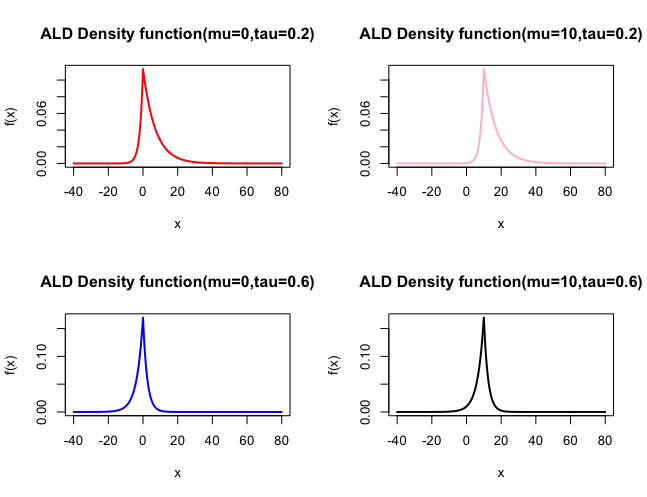
\includegraphics[width=0.8\textwidth]{Rplot01.png}
\caption{\label{fig:bar}ALD density functions with different location parameters and skewness parameters}
\end{figure}
\\
According to Kotz et.al 2001[2], we could represent the above as a Gaussian mixture form
\begin{equation*}
    Y=\mu+\xi_{\tau} U+\theta_{\tau} \sqrt{\delta U}Z
\end{equation*}
where $U$ follows an exponential distribution with the rate parameter $1/\theta$ and $Z$ is a random variable with a normal distribution with mean 0 and variance being 1. And we have $\xi_{\tau}=(1-2 \tau) /\{\tau(1-\tau)\}, \quad \theta_{\tau}=2 /\{\tau(1-\tau)\}$.

\section{Introduction to multivariate asymmetric Laplace distribution}
Based on the knowledge of the univariate AL, we can extend the result of asymmetric Laplace distribution to the multivariate Laplace distribution. For the multivariate asymmetric Laplace distribution we let the response variables, $\boldsymbol{Y}_{i}=\left(Y_{i 1}, \ldots, Y_{i p}\right)^{\top}$, to be the $p$-dimensional response variables with $i \in \{1,...,n\}$
entries for each response variable. From the details given in Kotz et.al 2001[2], for the $\boldsymbol{Y}_{i}$ which in the law of the multivariate asymmetric Laplace distribution with covariance matrix $\mathbf{\Sigma}$, and $K_{v}(\cdot)$ is the modified Bessel function of the third kind $v=(2-p)/2$. Thus we will have the following density function.
\begin{equation}
    g(\mathbf{y})=\frac{2}{(2 \pi)^{d / 2}|\mathbf{\Sigma}|^{1 / 2}}\left(\frac{\mathbf{y}^{\prime} \mathbf{\Sigma}^{-1} \mathbf{y}}{2}\right)^{v / 2} K_{v}\left(\sqrt{2 \mathbf{y}^{\prime} \mathbf{\Sigma}^{-1} \mathbf{y}}\right)
\end{equation}
Although we have the density function of the $p$-dimensional multivariate asymmetric Laplace distribution, we need to transform this density function into the alternative form, similar to the form we have discussed in the previous section. So now we can consider the following multivariate asymmetric Laplace distribution with density function from (Lea Petrella and Valentina Raponi,2019[3]),
\begin{equation}
    f_{Y}\left(\boldsymbol{y}_{i} \mid \boldsymbol{\beta}_{\tau} \boldsymbol{X}_{i}, \boldsymbol{D} {\xi}, \boldsymbol{D} {\Sigma} \boldsymbol{D}\right)=\frac{2 \exp \left\{\left(\boldsymbol{y}_{i}-\boldsymbol{\beta}_{\tau} \boldsymbol{X}_{i}\right)^{\top} \boldsymbol{D}^{-1} {\boldsymbol{\Sigma}}^{-1} {\xi}\right\}}{(2 \pi)^{p / 2}|\boldsymbol{D} {\Sigma} \boldsymbol{D}|^{1 / 2}}\left(\frac{{m}}{2+{d}}\right)^{v / 2} K_{v}\{\sqrt{(2+{d}) {m}}\}
\end{equation}
where $\beta_{\tau} \boldsymbol{X}_{i}$ is the location parameter vector, $\boldsymbol{D} {\xi} \in \mathbb{R}^{p}$ is the scale parameter, with ${\boldsymbol{D}}=\left[\begin{array}{ccc}\delta_{1} & 0 & 0 \\ 0 & \ddots & 0 \\ 0 & 0 & \delta_{n}\end{array}\right]$,
$\delta_{j}>0$,and ${\xi}=\left({\xi}_{1}, \ldots, {\xi}_{p}\right)^{\top},$ ${\xi}_{j}=\left(1-2 \tau_{j}\right) /\left\{\tau_{j}\left(1-\tau_{j}\right)\right\}$. 
${\boldsymbol{\Sigma}}$ is a $p \times p$ positive definite matrix such that ${\boldsymbol{\Sigma}}={\boldsymbol{\Lambda}} {\boldsymbol{\Psi}} {\boldsymbol{\Lambda}},$ with ${\boldsymbol{\Psi}}$ being a correlation matrix and
$\operatorname{{\boldsymbol{\Lambda}}} =\left[\begin{array}{ccc}\sigma_{1} & 0 & 0 \\ 0 & \ddots & 0 \\ 0 & 0 & \sigma_{n}\end{array}\right]$, where ${\sigma}_{j}^{2}=2 /\left\{\tau_{j}\left(1-\tau_{j}\right)\right\}$ for all $j \in\{1, \ldots, p\}$. Also, ${m}=\left(\boldsymbol{y}-\boldsymbol{\beta}_{\tau} \boldsymbol{X}_{i}\right)^{\top}(\boldsymbol{D} {\boldsymbol{\Sigma}} \boldsymbol{D})^{-1}\left(\boldsymbol{y}-\boldsymbol{\beta}_{\tau} \boldsymbol{X}_{i}\right)$, ${d}=\boldsymbol{{\xi}}^{\top} \boldsymbol{{\Sigma}} \boldsymbol{{\xi}}$. Here we can also turn this into the Gaussian mixture form,
\begin{equation}
    \boldsymbol{Y}_{i}=\boldsymbol{\beta}_{\tau} \boldsymbol{X}_{i}+\boldsymbol{D} \boldsymbol{{\xi}} W+\sqrt{W} \boldsymbol{D} \boldsymbol{{\Sigma}}^{1 / 2} \boldsymbol{Z},
\end{equation}
 where $W$ is an exponentially distributed random variable with mean 1, independent from $\boldsymbol{Z}$, and $\boldsymbol{Z}$ is a $p$-dimensional standard normal distribution. We also have the constrains as the univariate case, ${\xi}_{j}=\left(1-2 \tau_{j}\right) /\left\{\tau_{j}\left(1-\tau_{j}\right)\right\} \quad$ and $\quad {\sigma}_{j}^{2}=2 /\left\{\tau_{j}\left(1-\tau_{j}\right)\right\}$.
\section{Plan}
A brief review on the Bayesian statistics and the quantile regression will be given in Chapter 2. We will also discuss the relationship between the SMAL and the quantile regression in that Chapter. The dependence structure of the SMAL will be presented in Chapter 3 and the simulation study will be provided in Chapter 4. And Chapter 5 contains the real dataset application and the testing between it and the SMAL. Finally, the conclusion follows in Chapter 6.




%%%%%%%%%%%%%%%%%%%%%%%%%%%%%%%%%%%%%%%%%%%%%%%%%%%%%%%%%%%%%%%%%%%%
\chapter{Bayesian Statistics And Quantile Regression}
%%%%%%%%%%%%%%%%%%%%%%%%%%%%%%%%%%%%%%%%%%%%%%%%%%%%%%%%%%%%%%%%%%%%
Bayesian statistics, named after Thomas Bayes, is a statistical theory based on Bayesian probability interpretation, in which probability represents the credibility of events. Bayesian statistics use the Bayes' theorem to find the probability or credibility after being given a new data, assuming we already have some knowledge of the given data according to our prior experience or the results from previous experiments.

\section{Bayes' theorem}
First, we need to talk about the Bayes' theorem in a detailed way.
Bayes' theorem is about the conditional probability and the marginal probability of random events, A and B. And $\mathrm{P}(\mathrm{A} \mid \mathrm{B})$ is the probability that A occurs when B is given. We know that if B is given, the probability of event A will occur should be $P(A \mid B)=\frac{P(A \cap B)}{P(B)}$. Similarly, if A is given, the probability that B will occur should be $P(B \mid A)=\frac{P(A \cap B)}{P(A)}$. From these two we have $P(A \cap B)=P(A \mid B)^{*} P(B)=P(B \mid A)^{*} P(A)$. Therefore, we will reach the formula of the Bayes' theorem $P(A \mid B)=\frac{P(A \cap B)}{P(B)}=\frac{P(B \mid A)^{*} P(A)}{P(B)}$.



\section{Posterior distribution and Likelihood function}
In the Bayesian statistics, the posterior probability of a random or uncertain event is the conditional distribution which is based on our prior knowledge or the experience from previous work. From (Christopher M. Bishop (2006)[4]), we have the definition of the posterior distribution.
The posterior probability is the probability of the parameters $\theta$ given the evidence $X: p(\theta \mid X)$. The prior probability of $\theta$ is $p(\theta)$, and the observations $X = (x_1,...,x_n)$ have the likelihood $p(x \mid \theta)$, then the posterior probability can be calculated as the following:
\begin{equation}
    p(\theta \mid x)=\frac{p(x \mid \theta)}{p(x)} p(\theta)
\end{equation}
Since we can consider $p(x) = \int_{\Theta} f(\mathbf{X} \mid \theta) p(\theta) d \theta$ as a constant. Therefore, we can write the posterior probability distribution as 
Posterior probability $\propto$ Likelihood $\times$ Prior probability.\\
Likelihood function is a joint density function of each observations of $X$, say, if $\boldsymbol{X} = (x_1,...,x_n)$ has a joint density function $f\left(x_{1}, x_{2}, \ldots, x_{n} \mid \theta\right)$, then the likelihood function with respect to $\theta$ can be written as
\begin{equation}
    L(\theta)=L\left(\theta \mid x_{1}, x_{2}, \ldots, x_{n}\right)=f\left(x_{1}, x_{2}, \ldots, x_{n} \mid \theta\right),
\end{equation}
if $X_{1}, X_{2}, \ldots, X_{n}$ are i.i.d., then $L(\theta)=\prod_{i=1}^{n} f\left(x_{i} \mid \theta\right)$.
\section{Quantile regression}
Before talking about the quantile regression, we need to review the regression analysis. Including the linear regression, polynomial regression, most of regression analysis, we first assume the data from some fixed function and let the function fit the data to find the unknown parameters. We often use the MSE to let the function fit more data, where
$M S E=\frac{1}{n} \sum_{i=1}^{n}\left(y_{i}-\hat{f}\left(x_{i}\right)\right)^{2}=E(y-\hat{f}(x))^{2}$. Actually, we have got the expectation of $Y$. Hence, we can conclude from those analysis, in essence, the function obtained by all regression analysis is a conditional expectation function,i.e., in the condition of fixed $x$ to find the expectation of $Y$. \\
Now we introduce the quantile regression which focuses on not only the expectation of $Y$, but also the whole distribution of $Y$. According to the seminal work by Koenker and Bassett(R. Koenker, G. Bassett Jr,1978[5]), quantile regression has been recognized in recent years as a robust statistical procedure that offers a powerful alternative to ordinary mean regression. While standard regression methods usually focus on modelling the conditional mean of the response variable, quantile regression models the conditional median or other quantiles of the response variable. From(Geraci M and Bottai M.,2007[1]), if we have a data in the form of $\left(\mathbf{x}_{i}^{\mathrm{T}}, y_{i}\right),$ for $i=1, \ldots, N$ where $y_{i}$ are independent scalar observations of a continuous random variable with common cumulative distribution function $F_{y},$ whose shape is not exactly known, and $\mathbf{x}_{i}^{\mathrm{T}}$ are row $p$ -vectors of a known design matrix $X$. The linear conditional quantile functions are defined as $G_{y_{i}}\left(\tau \mid \mathbf{x}_{i}\right)=\mathbf{x}_{i}^{\mathrm{T}} \beta, \quad i=1, \ldots, N$ with $\tau \in (0,1)$ being the quantile, $G_{y_{i}}(\cdot) \equiv F_{y_{i}}^{-1}(\cdot),$ and $\beta \in \mathbb{R}^{p}$ is a column vector of length $p$ with unknown fixed parameters. We can minimize the following equation to find the quantile
\begin{equation}
\begin{split}
     \hat{Q}_{Y}(\tau) & =\operatorname{argmin}_{\xi_{\tau} \in R}\left(\sum_{i: Y_{i}>\xi_{\tau} } \tau\left|Y_{i}-\xi_{r}\right|+\sum_{i: Y_{i}<\xi_{\tau}  }(1-\tau)\left|Y_{i}-\xi_{r}\right|\right)\\
     \min _{\beta \in \mathbb{R}^{p}} V_{N}(\beta), V_{N}(\beta) & = \sum_{i \in\left(i: y_{i} \geqslant \mathbf{x}_{i}^{\mathrm{T}} \beta\right)}^{N} \tau\left|y_{i}-\mathbf{x}_{i}^{\mathrm{T}} \beta\right|+\sum_{i \in\left(i: y_{i}<\mathbf{x}_{i}^{\mathrm{T}} \beta\right)}^{N}(1-\tau)\left|y_{i}-\mathbf{x}_{i}^{\mathrm{T}} \beta\right|,
\end{split}
\end{equation}
yields
\begin{equation}
    \beta_\tau = \operatorname{argmin}_{\beta\in \mathbb{R}^p}\left(\sum_{i \in\left(i: y_{i} \geqslant \mathbf{x}_{i}^{\mathrm{T}} \beta\right)}^{N} \tau\left|y_{i}-\mathbf{x}_{i}^{\mathrm{T}} \beta\right|+\sum_{i \in\left(i: y_{i}<\mathbf{x}_{i}^{\mathrm{T}} \beta\right)}^{N}(1-\tau)\left|y_{i}-\mathbf{x}_{i}^{\mathrm{T}} \beta\right|\right),
\end{equation}

\section{Quantile regression and SMAL distribution}
The basic notion of the SMAL distribution has been discussed in Chapter 1. Now we will consider what is the relationship between the SMAL and the quantile regression and why does the SMAL is so used in practical. \\
For the univariate case first. In [3], let $\mathcal{Q}_{y_{i}}\left(\tau \mid \boldsymbol{x}_{i}\right)$ denote the quantile regression function of $y_i$ given $\boldsymbol{x}_{i}$ with the quantile parameter $\tau \in (0,1)$. Thus the quantile function can be modified as 
\begin{equation}
    \mathcal{Q}_{y_{i}}\left(\tau \mid \boldsymbol{x}_{i}\right)=\boldsymbol{x}_{i}^{\top} \boldsymbol{\beta}_{\tau}
\end{equation}
where $\boldsymbol{x}_{i}$ is a $k \times 1$ vector, and $\boldsymbol{\beta}_{\tau}$ is a $k \times 1$ vector of regression coefficients. Thus 
\begin{equation}
    y_{i}=\boldsymbol{x}_{i}^{\top} \boldsymbol{\beta}_{\tau}+\epsilon_{i}
\end{equation}
Therefore,the error term gives us a zero $\tau$-quantile,i.e., $\tau = 0$ thus from the equation (2.3.2) we obtain 
\begin{equation}
\begin{split}
    \beta_\tau & = \operatorname{argmin}_{\beta\in \mathbb{R}^k}\left(\sum_{i \in\left(i: y_{i} \geqslant \mathbf{x}_{i}^{\mathrm{T}} \beta\right)}^{N} \tau\left|y_{i}-\boldsymbol{x}_{i}^{\top} \boldsymbol{\beta}_{\tau}\right|+\sum_{i \in\left(i: y_{i}<\mathbf{x}_{i}^{\mathrm{T}} \beta\right)}^{N}(1-\tau)\left|y_{i}-\boldsymbol{x}_{i}^{\top} \boldsymbol{\beta}_{\tau}\right|\right)\\
    & = \operatorname{argmin}_{\beta\in \mathbb{R}^k}\left(\sum_{i \in\left(i: y_{i}<\mathbf{x}_{i}^{\mathrm{T}} \beta\right)}^{N}(1-0)\left|y_{i}-\boldsymbol{x}_{i}^{\top} \boldsymbol{\beta}_{\tau}\right|\right)\\
    & = \operatorname{argmin}_{\beta\in \mathbb{R}^k} \sum_{i=1}^{n} \rho_{\tau}\left(y_{i}-\boldsymbol{x}_{i}^{\top} \boldsymbol{\beta}_{\tau}\right)
\end{split}
\end{equation}
where $\rho_\tau$ is a loss function.\\
Next, we move to the multivariate case from([3]). $\boldsymbol{\beta}_{\tau}$ has become a $p \times k$ matrix of the regression coefficients.
\begin{equation}
\left[\begin{array}{c}
\mathcal{Q}_{Y_{i 1}}\left(\tau_{1} \mid \boldsymbol{X}_{i}\right) \\
\vdots \\
\mathcal{Q}_{Y_{i p}}\left(\tau_{p} \mid \boldsymbol{X}_{i}\right)
\end{array}\right]=\boldsymbol{\beta}_{\tau} \boldsymbol{X}_{i},
\end{equation}
where $\mathcal{Q}_{Y_{i j}}\left(\tau_{j} \mid \boldsymbol{X}_{i}\right)$ denotes the $\tau_{j}$ -level quantile regression function of $Y_{i j}$ given $\boldsymbol{X}_{i} .$
Since the quantile regression can provide us the whole distribution of the dataset without knowing its shape, namely, non-parametric. And the SMAL has a direction definition based on the quantiles which can be applied directly to the quantile regression analysis. And in practice, when we are given a data, without any prior knowledge of the shape of the data, we thus cannot apply the common linear regression or polynomial regression. This makes the scale-generalized multivariate asymmetric Laplace distribution a widely used distribution to fit the real data.
%%%%%%%%%%%%%%%%%%%%%%%%%%%%%%%%%%%%%%%%%%%%%%%%%%%%%%%%%%%%%%%%%%%%
\chapter{Copula}
%%%%%%%%%%%%%%%%%%%%%%%%%%%%%%%%%%%%%%%%%%%%%%%%%%%%%%%%%%%%%%%%%%%%
The very important tool we are using in the thesis is copula. When given a multivariate distribution, we can transform the density distribution into the copula form which can help us separate the marginal distributions from the dependency structure.(Martin Haugh,2016[6]). Especially, we can talk more about the research on the measurement on the association between variables, including the Spearman's $\rho$ and the tail dependence coefficients, those we will explain detailedly in Chapter 4.

\section{Introduction to Copulas}
Following(Thorsten Schmidt, 2006[7]), we have a definition of the $d$- dimensional copula. A $d$-dimensional copula $C$: $[0,1]^{p}: \rightarrow[0,1]$ is a function which is a cumulative distribution function with uniform marginals. Assume we have a uniform distribution $U \sim U[0,1]$, $F_X$ is a continuous CDF of X, thus
$P\left(F^{\leftarrow}(U) \leq x\right)=F_{X}(x)$ and the inverse function should be,
$F_{X}(X) \sim U[0,1]$. Given a $p$-variate vector $\mathbf{X}=\left(X_{1}, \ldots, X_{p}\right)$ with CDF $F_X$ and continuous and increasing marginals, thus $F_{X_{1}}\left(X_{1}\right), \ldots, F_{X_{p}}\left(X_{p}\right)$ is a copula, we can denote it by $C_X$, and
\begin{equation}
    \begin{aligned} C_{X}\left(u_{1}, \ldots, u_{p}\right) &=P\left(F_{X_{1}}\left(X_{1}\right) \leq u_{1}, \ldots, F_{X_{p}}\left(X_{d}\right) \leq u_{p}\right) \\ &=P\left(X_{1} \leq F_{X_{1}}^{-1}\left(u_{1}\right), \ldots, X_{p} \leq F_{X_{p}}^{-1}\left(u_{p}\right)\right) \\ &=F_{\mathbf{X}}\left(F_{X_{1}}^{-1}\left(u_{1}\right), \ldots, F_{X_{p}}^{-1}\left(u_{p}\right)\right) \end{aligned},
\end{equation}
if we let $u_{i}:=F_{X_{i}}\left(x_{i}\right)$ for $i \in \{1,...,p\}$, then
\begin{equation}
F_{\mathbf{X}}\left(x_{1}, \ldots, x_{d}\right)=C_{X}\left(F_{X_{1}}\left(x_{1}\right), \ldots, F_{X_{p}}\left(x_{p}\right)\right)
\end{equation}
And Equation (3.1.2) gives us the Sklar's Theorem.
\section{Copulas in this thesis}
In this thesis, we will use three typical copulas, the Gaussian copula the Clayton copula, and the Gumbel copula. 
First, we introduce the Gaussian copula. The Gaussian copula is a transformation of the multivariate Gaussian distribution, i.e., the Gaussian copula is a distribution over the unit cube $[0,1]^d$ which is constructed from the $d$-dimensional multivariate normal distribution. We use the Gaussian copula instead of the bivariate normal because of its generality.\\
And the Clayton and Gumbel copulas are bivariate copulas, called the Archimedean copula(Nelsen, R. B. (2006)[8]). Archimedean copulas admit an explicit formula, which is, sometimes, not possible for the Gaussian copula. And we have the following explicit expression of the Clayton copula(Clayton, David G.,1978[9]) and the Gumbel copula
\begin{equation}
\begin{array}{|l|l|l|}
\hline \text { Clayton } & {\left[\max \left\{u^{-\theta}+v^{-\theta}-1 ; 0\right\}\right]^{-1 / \theta}} & \theta \in[-1, \infty) \backslash\{0\} \\
\hline \text { Gumbel } & \exp \left[-\left((-\log (u))^{\theta}+(-\log (v))^{\theta}\right)^{1 / \theta}\right] & \theta \in[1, \infty) \\
\hline
\end{array}
\end{equation}
From the defination equation of the Clayton copula, we can tell when $\theta \rightarrow 0$ we obtain the independence copula, and when $\theta \rightarrow \infty$ the Clayton copula becomes the comonotonicity copula. Also, considering the Gumbel copula, for $\theta=1$ we reach the independence copula, then when $\theta \rightarrow \infty$ the Gumbel copula becomes the comonotonicity copula(Thorsten Schmidt,2006[7]).
The following figures gives us the density plots and the scatter plots of the Gaussian copula, Clayton copula, and Gumbel copula.
\begin{figure}[h]
\begin{subfigure}{.5\textwidth}
  \centering
  % include first image
  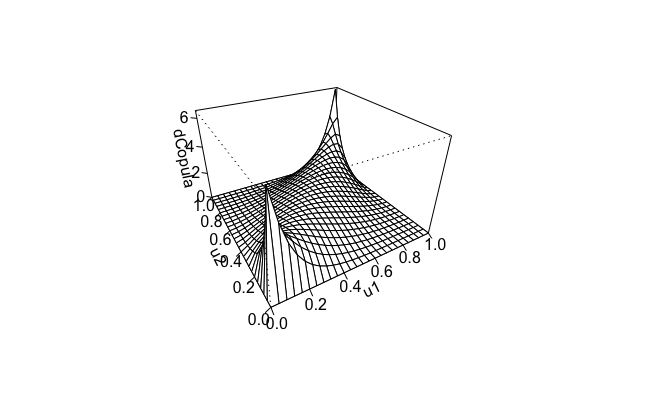
\includegraphics[width=\linewidth,height=4cm]{gaussiand.png}  
  \caption{density plot of Gaussian copula with $\rho=0.8$}
  \label{fig:sub-first}
\end{subfigure}
\begin{subfigure}{.5\textwidth}
  \centering
  % include second image
  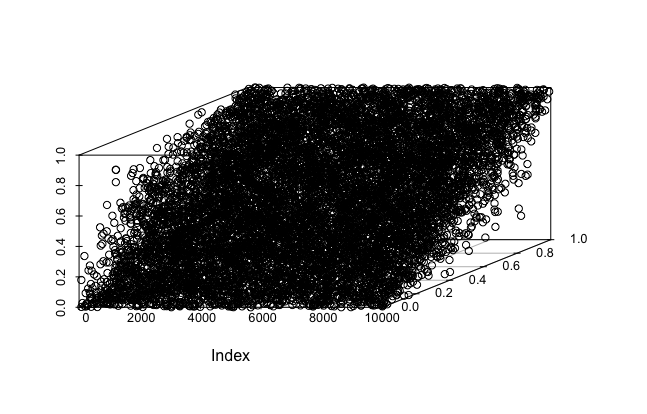
\includegraphics[width=\linewidth,height=4cm]{gaussainr.png}  
  \caption{scatter plot of Gaussian copula with $\rho=0.8$}
  \label{fig:sub-second}
\end{subfigure}
\begin{subfigure}{.5\textwidth}
  \centering
  % include third image
  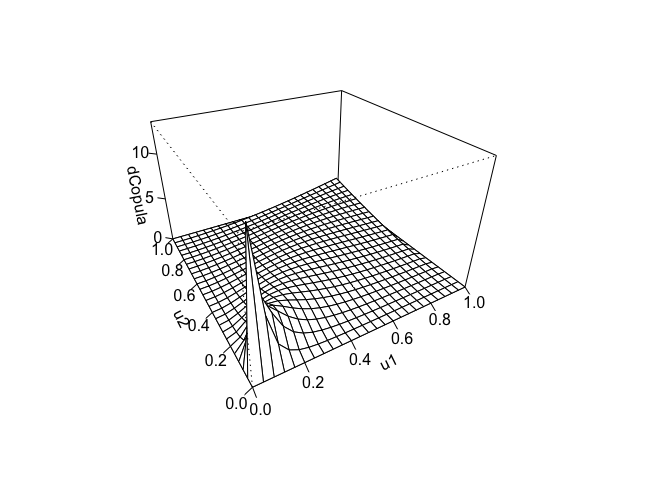
\includegraphics[width=\linewidth,height=4cm]{scattercc.png}  
  \caption{density plot of Clayton copula with $\theta=2$}
  \label{fig:sub-third}
\end{subfigure}
\begin{subfigure}{.5\textwidth}
  \centering
  % include forth image
  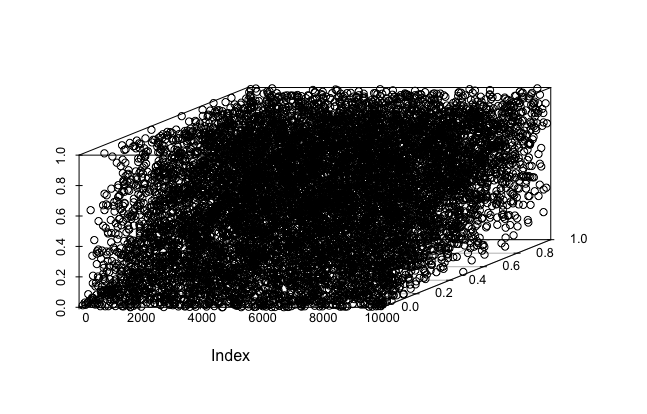
\includegraphics[width=\linewidth,height=4cm]{claytonr.png}  
  \caption{scatter plot of Clayton copula with $\theta=2$}
  \label{fig:sub-forth}
\end{subfigure}
\begin{subfigure}{.5\textwidth}
  \centering
  % include fifth image
  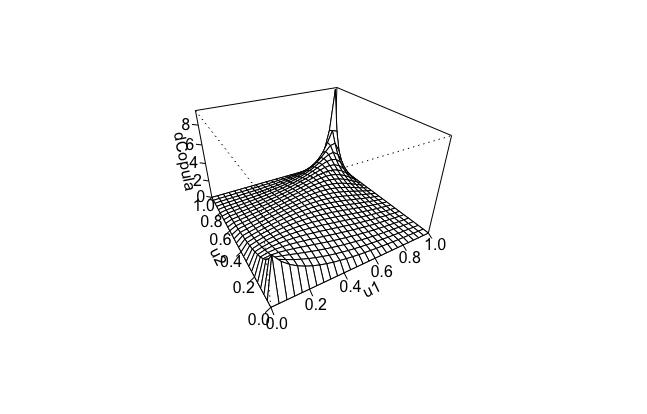
\includegraphics[width=\linewidth,height=4cm]{gumbeld.png}  
  \caption{density plot of Gumbel copula with $\theta=2$}
  \label{fig:sub-fifth}
\end{subfigure}
\begin{subfigure}{.5\textwidth}
  \centering
  % include sixth image
  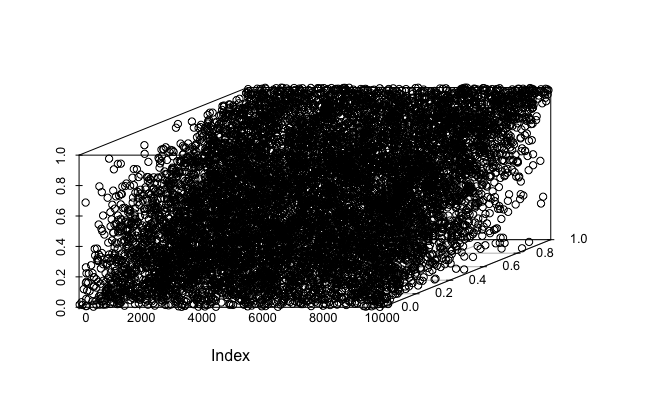
\includegraphics[width=\linewidth,height=4cm]{gumbelr.png}  
  \caption{scatter plot of Gumbel copula with $\theta=2$}
  \label{fig:sub-sixth}
\end{subfigure}

\end{figure}
\section{Frequentist and Bayesian statistics with respect to copulas}
It is possible to show (Clara Grazian and Brunero Liseo,2017[10]) that the density of a vector $\boldsymbol{X} = (X_1,..,X_p)$ has a copula representation in the continuous case, which is given by
\begin{equation}
f(x \mid \lambda, \theta)=c(u ; \theta) \prod_{j=1}^{p} f_{j}\left(x_{j} \mid \lambda_{j}\right).
\end{equation}
where $c(u;\theta)$ is the derivative with respect to $\theta$ of the $p$-dimensional function $C_X$ according to the equation (3.1.2). Since we have discussed the posterior distribution of the vector in section 2.2. Thus we can express the posterior as the following equation
\begin{equation}
\begin{split}
    \pi(\theta, \lambda \mid x) &\propto L(x \mid \lambda, \theta) \times \pi(\theta, \lambda) \\
     &\propto \prod_{j=1}^{p} f_{j}\left(x_{j} \mid \lambda_{j},\theta\right) \times \pi(\theta, \lambda)\\
     &\propto \pi(\theta, \lambda) \prod_{i=1}^{n}\left[c\left(u_{i} ; \theta\right) \prod_{j=1}^{p} f\left(x_{i j} ; \lambda_{j}\right)\right]
\end{split}
\end{equation}
The most difference between frequentist statistics and Bayesian statistics is the way we treat a data. For the frequentist statistics, all the estimations of the parameters are based on the original data itself. The frequentist method interprets the probability as a statistical mean by applying a huge number of independent experiments, while, the Bayesian method would rely on the prior of the parameter. Thus compared with the frequentist methods, the Bayesian method is more flexible since it assumes the parameter has a prior distribution instead of being a fixed value, especially, for the non-parametric case. In the parametric case, the estimations from the frequentist methods are based on maximizing the value of $\theta$ and $\lambda$ from the likelihood estimation, i.e., the MLE of those parameters. (Joe,2015[11]) However, for the Bayesian method, the joint posterior distribution will be evaluated by the Monte Carlo algorithm with $\theta$, and $(\lambda_1,..,\lambda_p)$ generated separately by using a Gibbs sampling(Clara Grazian and Brunero Liseo,2017[10]). Therefore, we have another way to look back at the frequentist statistics and Bayesian statistics. For the most of the time, the frequentist change the problem into an optimization problem while the Bayesian method will change the same problem into the sampling problem. This is the biggest difference between these two methods.
%%%%%%%%%%%%%%%%%%%%%%%%%%%%%%%%%%%%%%%%%%%%%%%%%%%%%%%%%%%%%%%%%%%%
\chapter{The dependence structure of the SMAL}\label{cha}
%%%%%%%%%%%%%%%%%%%%%%%%%%%%%%%%%%%%%%%%%%%%%%%%%%%%%%%%%%%%%%%%%%%%
Now we are moving to the dependence structure of the SMAL distribution. To talk about the dependence structure we need consider two factors, Spearman's rho and the tail dependence coefficients.

\section{Spearman's rho}
Spearman's rho is also called Spearman's rank correlation coefficient, it is statistical parameter which is widely used in the non-parametric cases for the measurement of dependence between the rankings of two variables. For the bivariate case, the definition of the Spearman's rho is given by 
\begin{equation}
\rho_n:=\operatorname{Corr}\left(F_{1}\left(X_{1}\right), F_{2}\left(X_{2}\right)\right)
\end{equation}
where $F_1, F_2$ are the marginals of two random variable $X_1,X_2$, respectively.(Thorsten Schmidt,2006[7]).\\
Let $X$ and $Y$ be continuous random variables with the distribution functions $F$ and $G$, respectively. And in the copula representation, $u = F(x)$ and $v = G(y)$. Therefore, the Spearman's $\rho$ in terms of $C(u,v)$ is given by (Schweizer and Wolff, 1981[12])
\begin{equation}
\begin{split}
\rho &=12 \int_{0}^{1} \int_{0}^{1}(C(u, v)-u v) d u d v\\
& = 12 \int_{0}^{1} \int_{0}^{1}C(u, v)d u d v -12 \int_{0}^{1} \int_{0}^{1}u v d u d v\\
& = 12 \int_{0}^{1} \int_{0}^{1}C(u, v)d u d v - 3.
\end{split}
\end{equation}
Now we will estimate the Spearman's $\rho$, which means we need to find the posterior distribution of the Spearman's $\rho$, say, $\hat{\rho}$.
(Clara Grazian and Brunero Liseo,2017[10])) gives us an estimation of Spearman's $\rho$ which is given by
\begin{equation}
\hat{\rho}_{n}=\frac{1}{n} \sum_{i=1}^{n}\left(\frac{12}{n^{2}-1} R(x_i) R(y_i)\right)-3 \frac{n+1}{n-1},
\end{equation}
where 
\begin{equation}
R(x_i)=\operatorname{rank}\left(x_{i}\right)=\sum_{k=1}^{n} \mathbb{I}\left(x_{k} \leq x_{i}\right), \quad R(y_i)=\operatorname{rank}\left(y_{i}\right)=\sum_{k=1}^{n} \mathbb{I}\left(y_{k} \leq y_{i}\right), \quad i=1, \ldots, n.
\end{equation}
Here we can try to prove the equation (4.1.3)
\begin{equation}
\begin{split}
\rho=\frac{S_{x y}}{S_{x} S_{y}} &=\frac{\frac{1}{n} \sum_{i=1}^{n}\left(R\left(x_{i}\right)-\mathbb{E}(R(x))\right) \cdot\left(R\left(y_{i}\right)-\mathbb{E}(R(y))\right)}{\sqrt{\var(R(x))} \cdot\sqrt{\var(R(y))}}\\
& = \frac{\frac{1}{n} \sum_{i=1}^{n}\left(R\left(x_{i}\right)-\overline{R(x)}\right) \cdot\left(R\left(y_{i}\right)-\overline{R(y)}\right)}{\sqrt{\left(\frac{1}{n} \sum_{i=1}^{n}\left(R\left(x_{i}\right)-\overline{R(x)}\right)^{2}\right) \cdot\left(\frac{1}{n} \sum_{i=1}^{n}\left(R\left(y_{i}\right)-\overline{R(y)}\right)^{2}\right)}}\\
& = \frac{\frac{1}{n} \sum_{i=1}^{n} R\left(x_{i}\right) R\left(y_{i}\right)-\frac{1}{n} \cdot \frac{n+1}{2} \sum_{i=1}^{n} R\left(x_{i}\right)-\frac{1}{n} \cdot \frac{n+1}{2} \sum_{i=1}^{n} R\left(y_{i}\right)+\left(\frac{n+1}{2}\right)^{2}}{\frac{1}{n} \sum_{i=1}^{n}\left(R\left(x_{i}\right)\right)^{2}-\left(\frac{n+1}{2}\right)^{2}}\\
& = \frac{\frac{1}{n} \sum_{i=1}^{n} R\left(x_{i}\right) R\left(y_{i}\right)-\frac{n+1}{n} \sum_{i=1}^{n} R\left(x_{i}\right)+\left(\frac{n+1}{2}\right)^{2}}{\frac{1}{n} \cdot \frac{n(n+1)(2 n+1)}{6}-\left(\frac{n+1}{2}\right)^{2}}\\
& = \frac{\frac{1}{n} \sum_{i=1}^{n} R\left(x_{i}\right) R\left(y_{i}\right)-\frac{n+1}{n} \cdot \frac{n(n+1)}{2}+\left(\frac{n+1}{2}\right)^{2}}{\frac{n+1}{12}[2(2 n+1)-3(n+1)]}\\
& = \frac{\frac{1}{n} \sum_{i=1}^{n} R\left(x_{i}\right) R\left(y_{i}\right)-\frac{(n+1)^{2}}{2}+\frac{(n+1)^{2}}{4}}{\frac{n+1}{12}(4 n+2-3 n-3)}\\
& = \frac{1}{n} \sum_{i=1}^{n} R\left(x_{i}\right) R\left(y_{i}\right) \cdot \frac{12}{(n-1)(n+1)}-\frac{12}{(n-1)(n+1)} \frac{(n+1)^{2}(2-1)}{4}\\
& = \frac{12}{n\left(n^{2}-1\right)} \sum_{i=1}^{n} R\left(x_{i}\right) R(y_i)- 3 \cdot \frac{n+1}{n-1}\\
& = \hat{\rho}_{n}=\frac{1}{n} \sum_{i=1}^{n}\left(\frac{12}{n^{2}-1} R\left(x_{i}\right) R\left(y_{i}\right)\right)-3 \frac{n+1}{n-1}
\end{split}
\end{equation}
The frequentist method to find the estimator of the Spearman's $\rho$ is not directly computed, however, it can be found through the asymptotic variance of $\rho_n$ from(Borkowf,2002 [13]), that is
\begin{equation}
\sigma_{\mathrm{a}}^{2}\left(\hat{\rho}_{\mathrm{n}}\right)=144\left(-9 \phi_{1}^{2}+\phi_{3}+2 \phi_{4}+2 \phi_{5}+2 \phi_{6}\right)
\end{equation}
where
\begin{equation}
\begin{aligned}
\phi_{1} &=\mathbb{E}\left[F\left(X_{1}\right) G\left(Y_{1}\right)\right] \\
\phi_{2} &=\mathbb{E}\left[\left(1-F\left(X_{1}\right)\right)^{2}\left(1-G\left(Y_{1}\right)\right)^{2}\right] \\
\phi_{3} &=\mathbb{E}\left[\left(1-F(X_1)-G(Y_2)+H\left(X_{1}, Y_{2}\right)\right)\left(1-F\left(X_{2}\right)\right)\left(1-G\left(Y_{1}\right)\right)\right] \\
\phi_{4} &=\mathbb{E}\left[\left(1-F\left(\max \left\{X_{1}, X_{2}\right\}\right)\right)\left(1-G\left(Y_{1}\right)\right)\left(1-G\left(Y_{2}\right)\right)\right] \\
\phi_{5} &=\mathbb{E}\left[\left(1-F\left(X_{1}\right)\right)\left(1-F\left(X_{2}\right)\right)\left(1-G\left(\max \left\{Y_{1}, Y_{2}\right\}\right)\right)\right]
\end{aligned}
\end{equation}
with H being the joint distribution of $(X_1,Y_1)$ and $(X_2,Y_2)$, $F$ and $G$ being the marginal distribution of $X$ and $Y$, respectively.
Based on the knowledge above, we can apply the algorithm designed by (Clara Grazian and Brunero Liseo,2017[10]). 
\begin{algorithm}[H]
\SetAlgoLined
 Change the simulated data into the copula form\\
 Generate a sample of n pseudo-observations from the previous copula \\
 \begin{equation}
u=\left(\begin{array}{cc}
u_{11} & u_{12} \\
u_{21} & u_{22} \\
\cdots & \cdots \\
u_{n 1} & u_{n 2},
\end{array}\right)
\end{equation}
 (i)  \For {$b = 1 \rightarrow B$}{
     draw $\rho^{(b)}$ from the assumed prior distribution, such as $\rho^{(b)} \sim Unif(-1,1)$\\
     Compute a nonparametric estimate of the Spearman's $\rho$ :
     $\hat{\rho}_{n}=\frac{1}{n} \sum_{i=1}^{n}\left(\frac{12}{n^{2}-1} R\left(x_{i}\right) R\left(y_{i}\right)\right)-3 \frac{n+1}{n-1}$\\
     where $R(x_i)=\operatorname{rank}\left(x_{i}\right)$,$R(y_i)=\operatorname{rank}\left(y_{i}\right), i = 1,...,n$\\
     Compute the Bayesian exponentially tilted empirical likelihood
    } \\
 (ii)  \Return $\hat{\rho}_n$.
 \caption{Spearman's $\rho$ algorithm}
\end{algorithm} 
\section{Spearman's $\rho$ of the SMAL distribution and specific Copulas}
After introducing all the background knowledge, we can now start to find the first correlation coefficient, Spearman's $\rho$, of the SMAL distribution. To do this, we first need to simulate a SMAL distribution. Here we let the number of the Monte Carlo replications be 100, B = 100. The number of observations is 1000. And we use the bivariate asymmetric Laplace distribution instead of the multivariate Laplace distribution to get a conclusion without loss of generality and it will be easier for us to make comparison between the results from SMAL distribution and those three copulas. Hence the dimension parameter, $p=2$. And we call this simulated SMAL distribution, Y. Next, we need to change Y into the copula form in order to perform the algorithm. Since we obtained this Y with 100 replication, we thus got an array with 100 matrices and each matrix being $1000 \times 2$. Then we can make a scatter plot of one entry of the array of the pseudo-observations. 
\newpage
\begin{figure}[h]
\centering
  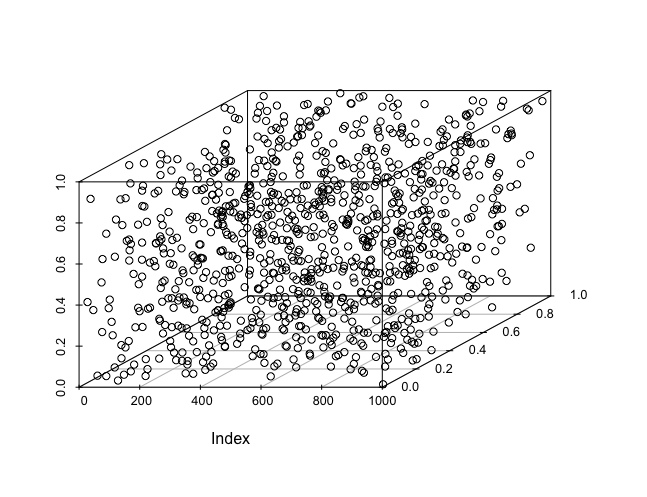
\includegraphics[width=12cm,height=10cm]{scatterSMAL.png}  
  \caption{Scatter plot of the uu[,,1]}
\end{figure}
The next step is applying the algorithm to find the posterior distributions of the Spearman's $\rho$ for both the SMAL distribution and the other three copulas. Therefore, we obtain the following density plots of those. \\
From those plots, we can tell, the concentration for the SMAL is around 0.2, while the concentrations for the other three copulas are around 0.5, 0.76, and 0.7 respectively. Since the closer the absolute value of Spearman's $\rho$ to 1, the better the correlation between two variables, the strength of the association of three copulas is much better than the SMAL distribution. However, the Spearman's $\rho$ is a non-parametric test, without having any prior knowledge or experience of the given data, it is acceptable to obtain such a 0.2 Spearman's $\rho$.
\newpage
\begin{figure}[h]
\begin{subfigure}{.5\textwidth}
  \centering
  % include first image
  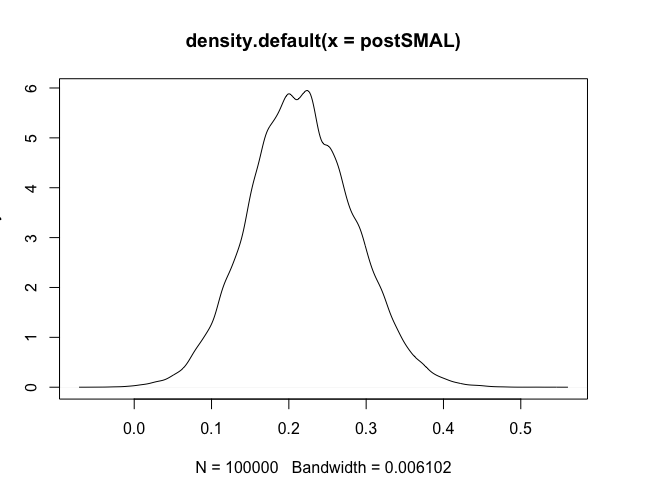
\includegraphics[width=\linewidth]{postSMAL.png}  
  \caption{density plot of the posterior distribution of Spearman's $\rho$ of the SMAL distribution}
  \label{fig:sub-first}
\end{subfigure}
\begin{subfigure}{.5\textwidth}
  \centering
  % include second image
  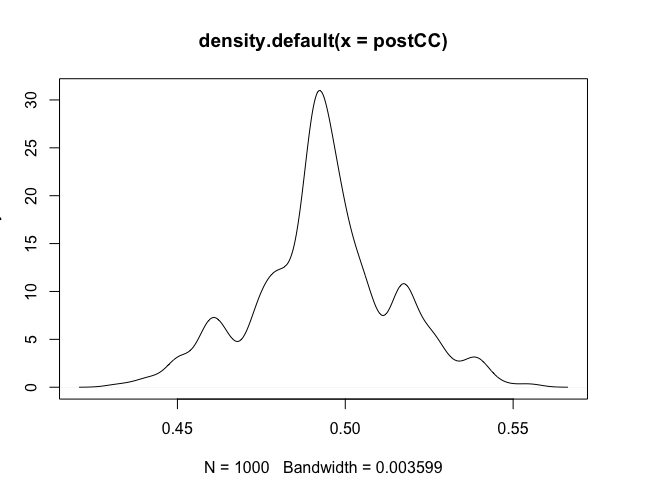
\includegraphics[width=\linewidth]{postCC.png}  
  \caption{density plot of the posterior distribution of Spearman's $\rho$ of the Clayton copula}
  \label{fig:sub-second}
\end{subfigure}

\begin{subfigure}{.5\textwidth}
  \centering
  % include third image
  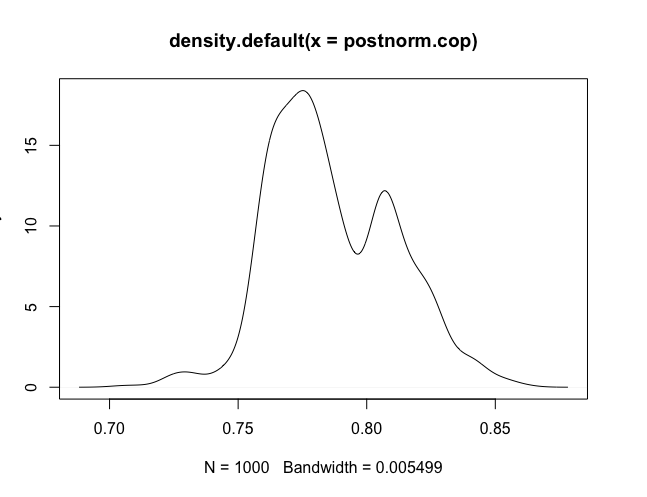
\includegraphics[width=\linewidth]{postGau.png}  
  \caption{density plot of the posterior distribution of Spearman's $\rho$ of the Gaussian copula}
  \label{fig:sub-third}
\end{subfigure}
\begin{subfigure}{.5\textwidth}
  \centering
  % include fourth image
  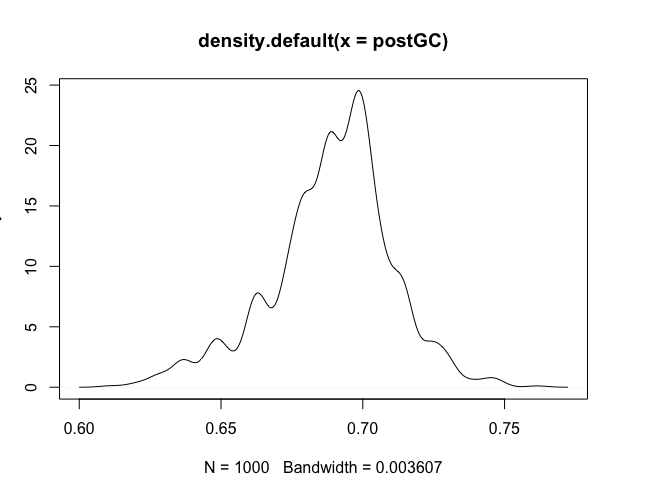
\includegraphics[width=\linewidth]{postGC.png}  
  \caption{density plot of the posterior distribution of Spearman's $\rho$ of the Gumbel copula}
  \label{fig:sub-fourth}
\end{subfigure}
\caption{Density plots of the posterior distributions of the Spearman's $\rho$ from different distributions}
\label{fig:fig}
\end{figure}
\section{Tail dependence coefficients}
Now we will introduce the tail dependence coefficients. Tail dependence coefficients measures the comovements in the tails of the distribution of two random variables (Hartmann, Philip et al, 2004[14]). We can divide the tail dependence coefficients into two parts, including the first part, the upper tail dependence coefficient, and the second part, lower tail dependence coefficient. When talking about the dependence structure of the multivariate distribution, especially the financial risk assessment it is very complicated to reach a conclusion. The reason is we can not only consider the correlation of the whole distribution or the financial derivative, but also consider the tail dependence of the asset price (Sibuya, 1959[15]). That is, the correlation between assets when a small probability event occurs.(An´e and Kharoubi ,2003[16]). Let us focus back on the definition of the tail dependence coefficients. The notion of the tail dependence is the connection with the extreme value on the data at the tail in the bivariate distribution. It is very convenient to build the connection between the tail dependence coefficients and copulas. \\
Here we can take the conditional probability,$P\left(X_{1}>x_{1} \mid X_{2}>x_{2}\right)$, into account again. We can interpret the conception of this conditional probability as: if we change the value of $X_2 >x_2$, does it affect the probability of $X_1>x_1$? And when the values of $x_1, x_2$ are large, it comes to the tail dependence of $X_1$, and $X_2$.\\
Let $C(u,v)$ be the copula function of $(X_1,X_2)$, where $u,v \in [0,1]$, thus we can easily obtain
\begin{equation}
P\left(X_{1}>x_{1} \mid X_{2}>x_{2}\right)=P\left(U_{1}>u_{1} \mid U_{2}>u_{2}\right).
\end{equation}
Besides, we have the survival function of copula of $X_1$ and $X_2$ from (Nelsen,2006[15])
\begin{equation}
\hat{C}\left(u_{1}, u_{2}\right)=u_{1}+u_{2}-1+C\left(1-u_{1}, 1-u_{2}\right)
\end{equation}
And the joint survival function $\bar{C}$ for two random variables which are uniformly $(0,1)$ distributed. Therefore, we have the following equation:
\begin{equation}
\begin{split}
\bar{C}\left(u_{1}, u_{2}\right)&=P\left(U_{1}>u_{1}, U_{2}>u_{2}\right)=1-u_{1}-u_{2}+C\left(u_1, u_{2}\right)\\
& = (1-u_1)+(1-u_2)-1+C(u_1,u_2)\\
& = \hat{C}(1-u_1, 1-u_2)
\end{split}
\end{equation}
Now assume $X$ and $Y$ be two continuous random variables with the marginals $F(X)$ and $G(Y)$, respectively. And the copula function of these two variable being $C(X,Y)$. Therefore, the upper and lower tail dependence coefficients are written as
\begin{equation}
\begin{split}
\lambda_{U}&=\lim _{u \rightarrow 1} P\left\{Y>G^{-1}(u) \mid X>F^{-1}(u)\right\}\\
&=\lim _{u \rightarrow 1} \frac{\hat{C}(1-u, 1-u)}{1-u}\\
&=\lim _{u \rightarrow 1^{-}} \frac{1-2 u+C(u,u)}{1-u},
    \end{split}
\end{equation}
and 
\begin{equation}
\begin{split}
\lambda_{L}&=\lim _{u \rightarrow 0} P\left\{Y<G^{-1}(u) \mid X<F^{-1}(u)\right\}\\
&=\lim _{u \rightarrow 0} \frac{C(u, u)}{u}.
\end{split}
\end{equation}
We will say $(X,Y)$ has upper and lower tail dependence when $\lambda_U$ and $\lambda_L$ are greater than 0, and upper and lower tail independence when $\lambda_U = 0$ and $\lambda_L = 0$.
Now if we want to apply the algorithm, we have to find the non-parametric estimator of $\lambda_U$ and $\lambda_L$. In (Frahm et al. 2005[17]), for the non-parametric case, the estimation of the tail dependence coefficients can be obtained from the empirical copula $\Tilde{C}_n$. And the empirical copula gives the following relationship
\begin{equation}
\Tilde{F}_{n}(x, y)=\Tilde{C}_{n}\left\{\Tilde{G}_{n}(x), \Tilde{H}_{n}(y)\right\}.
\end{equation}
The special case of non-parametric estimation given in (Joe et al. 1992[18]) is
\begin{equation}
\begin{split}
\hat{\lambda}_{U}&=2-\frac{1-\Tilde{C}_{n}((n-k) / n,(n-k) / n)}{1-(n-k) / n}\\
\hat{\lambda}_{L}&=\frac{\Tilde{C}_{n}\left(k/n, k/n\right)}{k/n}, \quad 0<k \leq n.
\end{split}
\end{equation}
And we have the following table, which gives us the tail dependence coefficients of the multivariate Archimedean copulas see(Salazar
and Ng, 2015[19])\\
\begin{tabular}{c|c|c|c} 
Copula & $C\left(u_{1}, \cdots, u_{d}\right)$ & $\lambda_{L}$ & $\lambda_{U}$ \\
\hline Clayton & $\left(1+\theta\left[\frac{1}{\theta} \sum_{j=1}^{d}\left(u_{j}^{-\theta}-1\right)\right]\right)^{-1 / \theta}$ & $d^{-1 / \theta}$ & 0 \\
Frank & $-\frac{1}{\theta} \log \left[1+\frac{\prod_{j=1}^{d}\left(\exp \left(-\theta u_{j}\right)-1\right)}{[\exp (-\theta)-1]^{d-1}}\right]$ & 0 & 0 \\
Gumbel & $\exp \left[-\left[\sum_{j=1}^{d}\left(-\log u_{d}\right)^{\theta}\right]^{1 / \theta}\right]$ & 0 & $\sum_{r=1}^{d}(-1)^{r+1}\left(\begin{array}{c}d \\
r\end{array}\right) r^{1 / \theta}$
\end{tabular}\\
We now can use the Bayesian estimates to find the posterior distribution of the tail dependence coefficients by presenting the density plots.
\begin{figure}[h]
\begin{subfigure}{.42\textwidth}
  \centering
  % include first image
  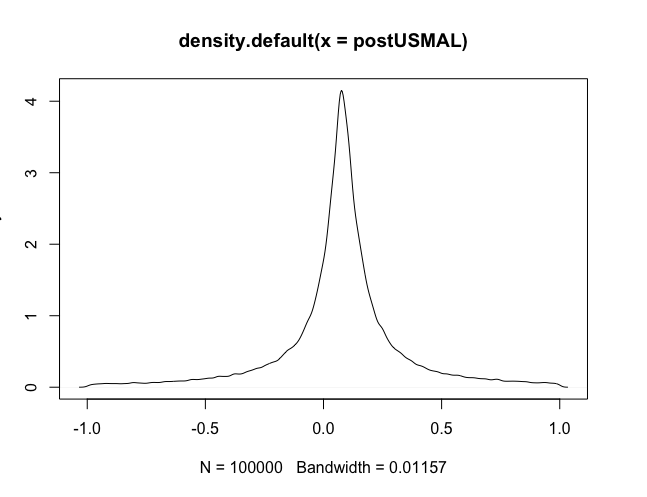
\includegraphics[width=\linewidth]{postUSMAL.png}  
  \caption{density plot of the posterior distribution of upper tail dependence coefficient of the SMAL distribution}
  \label{fig:sub-first}
\end{subfigure}
\begin{subfigure}{.42\textwidth}
  \centering
  % include second image
  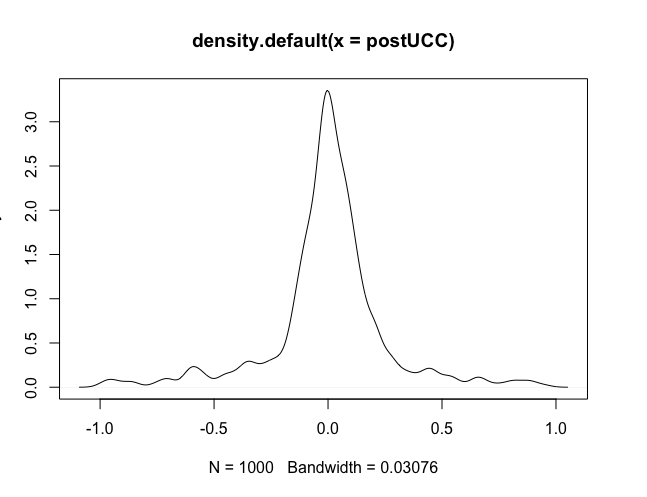
\includegraphics[width=\linewidth]{postUCC2.png}  
  \caption{density plot of the posterior distribution of upper tail dependence coefficient of the Clayton copula}
  \label{fig:sub-second}
\end{subfigure}

\begin{subfigure}{.42\textwidth}
  \centering
  % include third image
  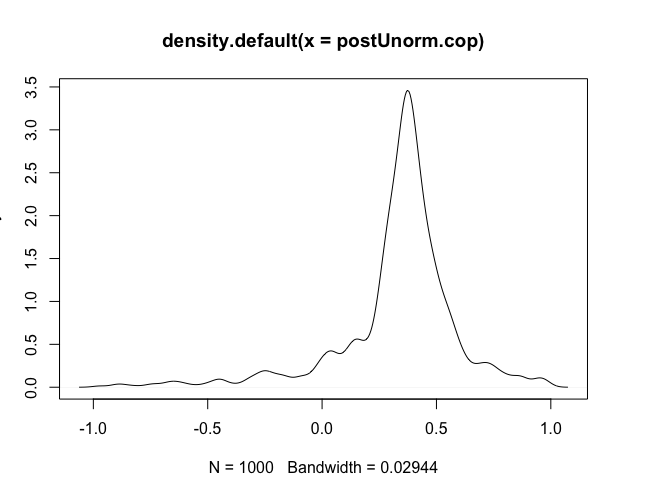
\includegraphics[width=\linewidth]{postUGau.png}  
  \caption{density plot of the posterior distribution of upper tail dependence coefficient of the Gaussian copula}
  \label{fig:sub-third}
\end{subfigure}
\begin{subfigure}{.42\textwidth}
  \centering
  % include fourth image
  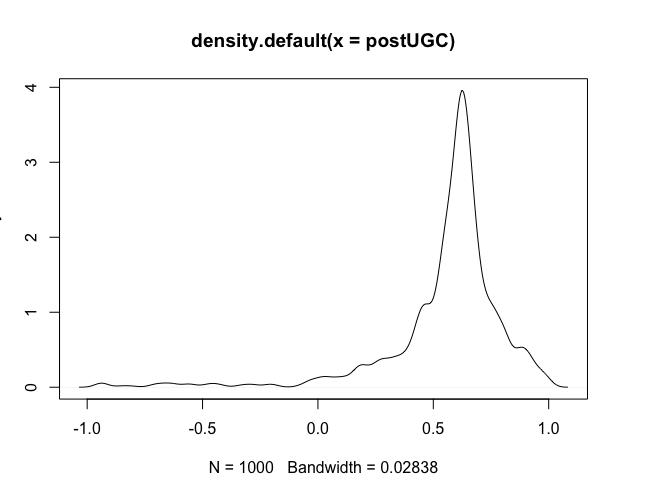
\includegraphics[width=\linewidth]{postUGC.png}  
  \caption{density plot of the posterior distribution of upper tail dependence coefficient of the Gumbel copula}
  \label{fig:sub-fourth}
\end{subfigure}
\caption{Density plots of the posterior distributions of upper tail dependence coefficients from different distributions in two dimensions.}
\label{fig:fig}
\end{figure}


\begin{figure}[h]
\begin{subfigure}{.42\textwidth}
  \centering
  % include first image
  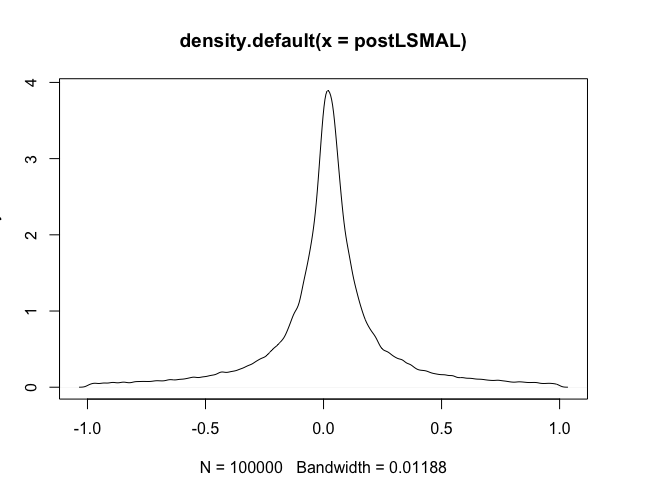
\includegraphics[width=\linewidth]{postLSMAL.png}  
  \caption{density plot of the posterior distribution of lower tail dependence coefficient of the SMAL distribution}
  \label{fig:sub-first}
\end{subfigure}
\begin{subfigure}{.42\textwidth}
  \centering
  % include second image
  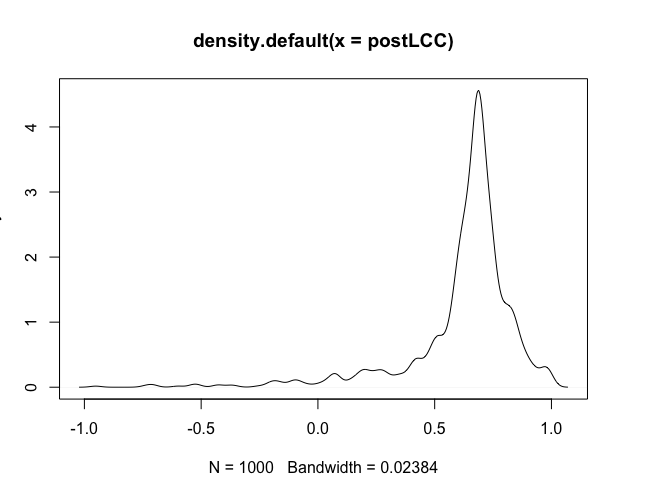
\includegraphics[width=\linewidth]{postLCC2.png}  
  \caption{density plot of the posterior distribution of lower tail dependence coefficient of the Clayton copula}
  \label{fig:sub-second}
\end{subfigure}

\begin{subfigure}{.42\textwidth}
  \centering
  % include third image
  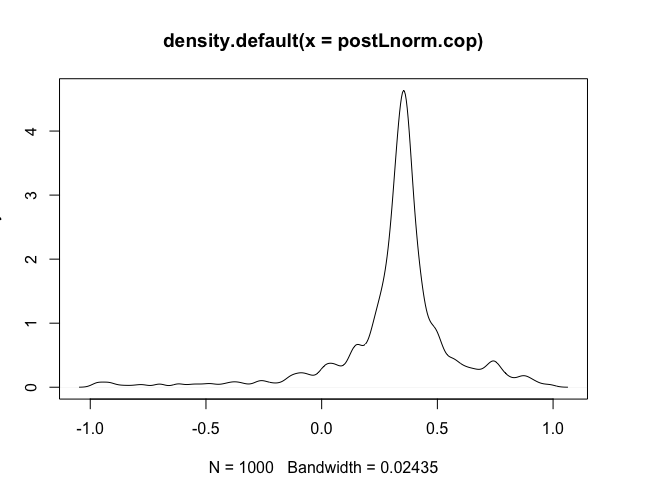
\includegraphics[width=\linewidth]{postLGau.png}  
  \caption{density plot of the posterior distribution of lower tail dependence coefficient of the Gaussian copula}
  \label{fig:sub-third}
\end{subfigure}
\begin{subfigure}{.42\textwidth}
  \centering
  % include fourth image
  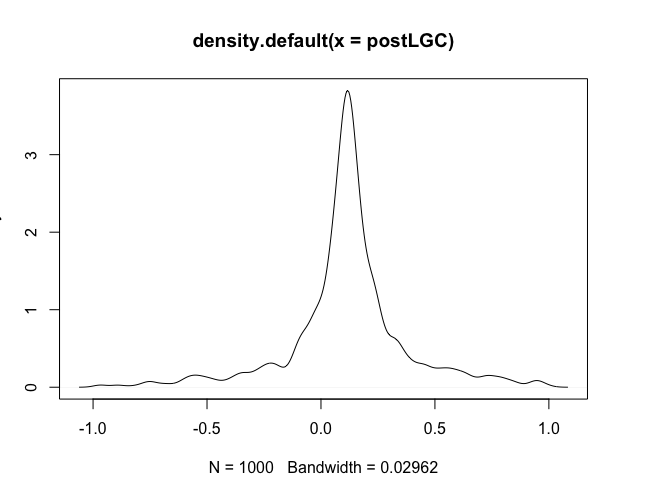
\includegraphics[width=\linewidth]{postLGC.png}  
  \caption{density plot of the posterior distribution of lower tail dependence coefficient of the Gumbel copula}
  \label{fig:sub-fourth}
\end{subfigure}
\caption{Density plots of the posterior distributions of lower tail dependence coefficients from different distributions in two dimensions.}
\label{fig:fig}
\end{figure}
From the figures above, we can tell both the upper and lower tail dependence coefficients of the SMAL distribution is concentrated around 0. For the Clayton copula, we can see that the upper tail dependence concentrates around 0 and the lower tail dependence  concentrates around 0.7 which match the expressions from (Salazar,2015), where $\lambda_U = 0$ and $\lambda_L = d^{-1/\theta}=2^{-1/2} = 0.707$. From the inspection of the Clayton we can find that the tail dependent coefficients found by the algorithm in this thesis is acceptable.\\
Overall, according to the Spearman's $\rho$ and the tail dependence coefficients, we can tell that the SMAL distribution is good for fit the data since it has a definition on quantiles first. And second, more events from the SMAL distribution will concentrate on the majority instead of being on the tail along with the acceptable Spearman's $\rho$.

%%%%%%%%%%%%%%%%%%%%%%%%%%%%%%%%%%%%%%%%%%%%%%%%%%%%%%%%%%%%%%%%%%%%
\chapter{Simulation Study}\label{ccl}
%%%%%%%%%%%%%%%%%%%%%%%%%%%%%%%%%%%%%%%%%%%%%%%%%%%%%%%%%%%%%%%%%%%%
In this chapter, we will move to the simulation study. To do this, I have changed the correlation matrix of the SMAL distribution and making other parameters fixed in order to see how the Spearman's $\rho$ and the tail dependence coefficients change. \\
Here we use the algorithm above with 1000 replications. By fixing a scale on a grid (between $-1$ and $1$), I will repeat the simulation and find the posterior distributions for the Spearman's $\rho$ and the tail dependence coefficients. \\
As is mentioned in Chapter 1, we know $\Psi$ is the correlation matrix. In our case, $\Psi$ is a $2 \times 2$ matrix, $\Psi=\left[\begin{array}{ccc}1 & a  \\ b & 1\end{array}\right]$, where we want to change a and b to change the correlation matrix. Here we are considering two cases, $a=b$ and $a=-b$. Since $a$ and $b$ are constrained in $[-1,1]$, thus we have the following scenarios in which the correlations are equal:
\begin{equation}
\begin{split}
\Psi_{g1}=\left[\begin{array}{ll}
1 & -1 \\
-1 & 1
\end{array}\right] \Psi_{g2}=\left[\begin{array}{ll}
1 & -0.5 \\
-0.5 & 1
\end{array}\right]\\ \Psi_{g3}=\left[\begin{array}{ll}
1 & 0 \\
0 & 1
\end{array}\right] \Psi_{g4}=\left[\begin{array}{ll}
1 & 0.5 \\
0.5 & 1
\end{array}\right] \Psi_{g5}=\left[\begin{array}{ll}
1 & 1 \\
1 & 1
\end{array}\right],
\end{split}
\end{equation}
and in which the correlations are the opposite:
\begin{equation}
\begin{split}
\Psi_{ng1}=\left[\begin{array}{ll}
1 & -1 \\
1 & 1
\end{array}\right] \Psi_{ng2}=\left[\begin{array}{ll}
1 & -0.5 \\
0.5 & 1
\end{array}\right]\\ \Psi_{ng3}=\left[\begin{array}{ll}
1 & 0 \\
0 & 1
\end{array}\right] \Psi_{ng4}=\left[\begin{array}{ll}
1 & 0.5 \\
-0.5 & 1
\end{array}\right] \Psi_{ng5}=\left[\begin{array}{ll}
1 & 1 \\
-1 & 1
\end{array}\right].
\end{split}
\end{equation}
Since $\Psi_{g3} = \Psi_{ng3}$, we will repeat four times of the simulations for the case that the correlations are in the opposite sign. The reason why we only change the value out of the diagonal is because the ones on the diagonal are associated with the variance, so there is not much effect on the dependence structure. 
\section{Simulation study on Spearman's $\rho$}
As what we have done before, we plot the density of the posterior distributions of Spearman's $\rho$ of two cases separately.
\newpage
\begin{figure}[h]
\begin{center}$
\begin{array}{lll}
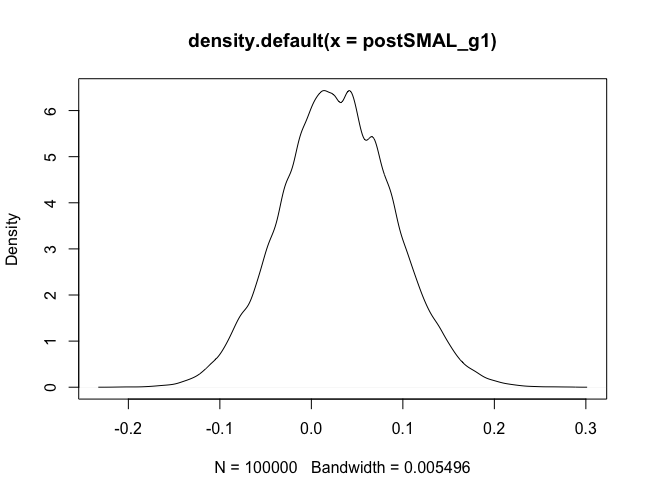
\includegraphics[width=50mm, height=35mm]{postSMAL_g1.png}&
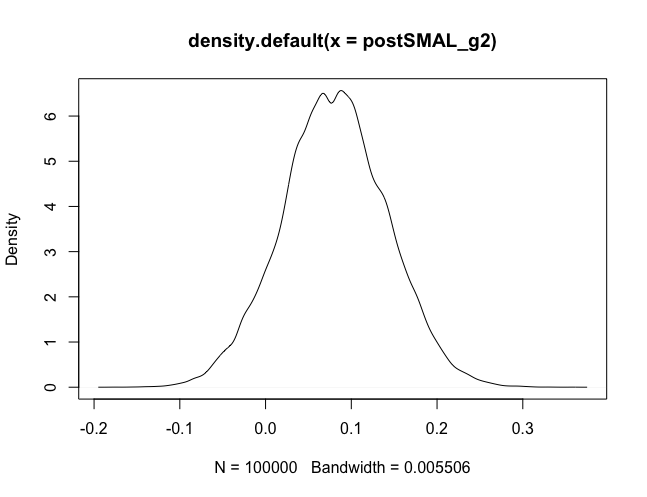
\includegraphics[width=50mm, height=35mm]{postSMALg2.png}&
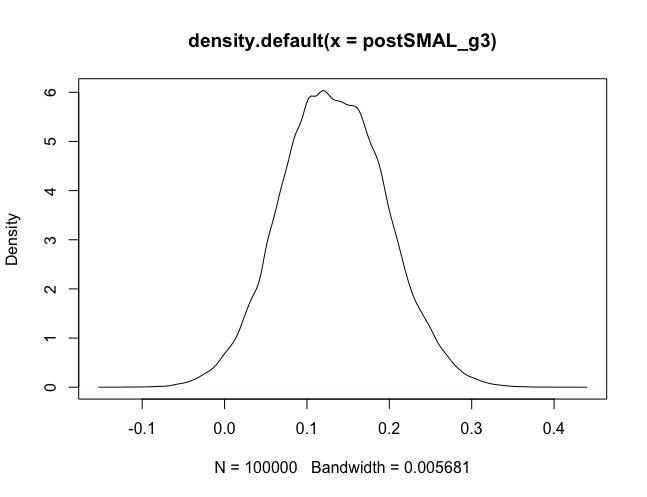
\includegraphics[width=50mm, height=35mm]{postSMALg3.png}
\end{array}$
\end{center}

\begin{center}$
\begin{array}{rr}
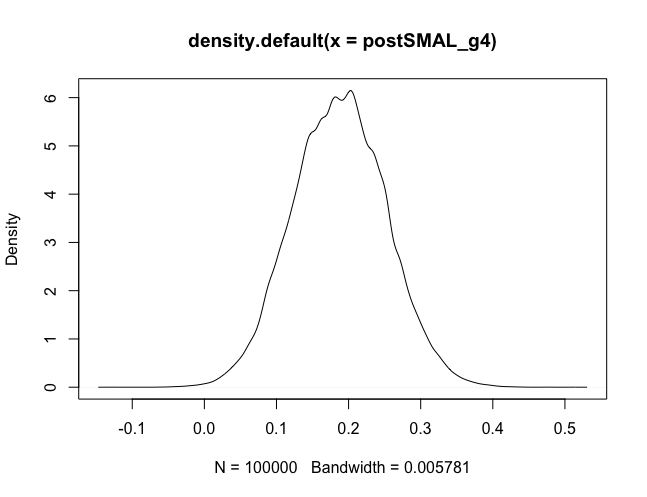
\includegraphics[width=50mm, height=35mm]{postSMALg4.png}&
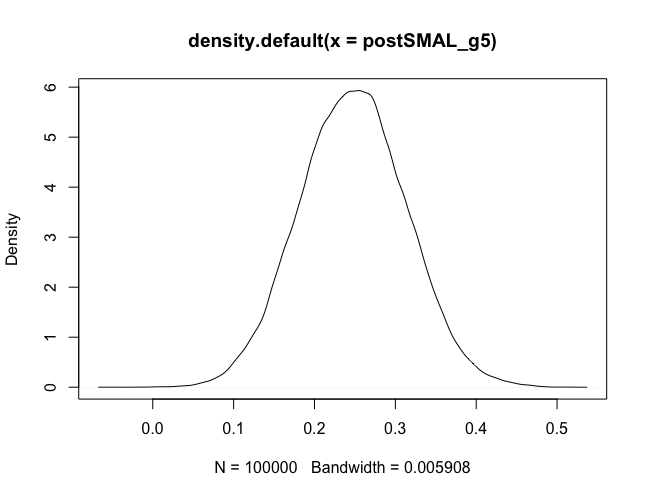
\includegraphics[width=50mm, height=35mm]{postSMALg5.png}
\end{array}$
\end{center}
\caption{Posterior distributions of Spearman's $\rho$ for the equal correlation.}
\label{pics:blablabla}
\end{figure}

\begin{figure}[h]
\centering
\begin{subfigure}{.32\textwidth}
  \centering
  % include first image
  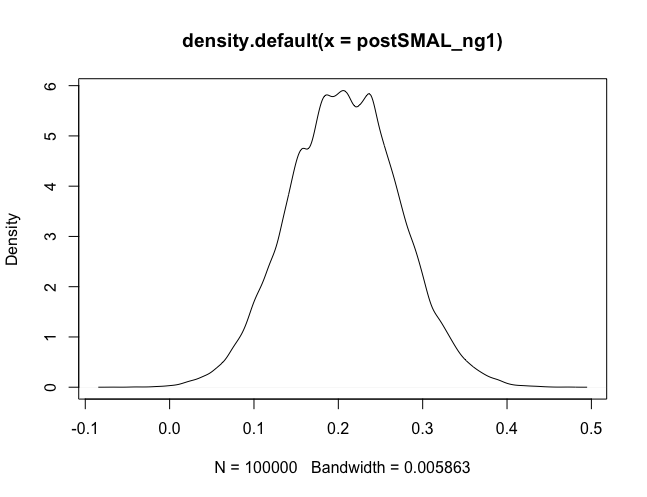
\includegraphics[width=\linewidth]{postSMALng1.png}  
  \label{fig:sub-first}
\end{subfigure}
\begin{subfigure}{.32\textwidth}
  \centering
  % include second image
  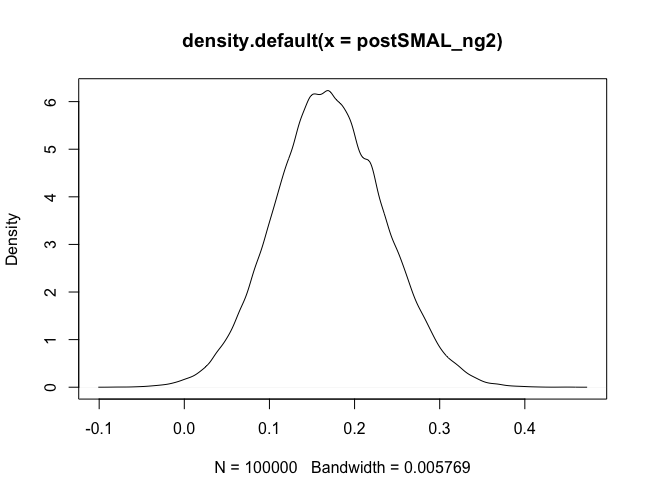
\includegraphics[width=\linewidth]{postSMALng2.png}  
  \label{fig:sub-second}
\end{subfigure}

\begin{subfigure}{.32\textwidth}
  \centering
  % include third image
  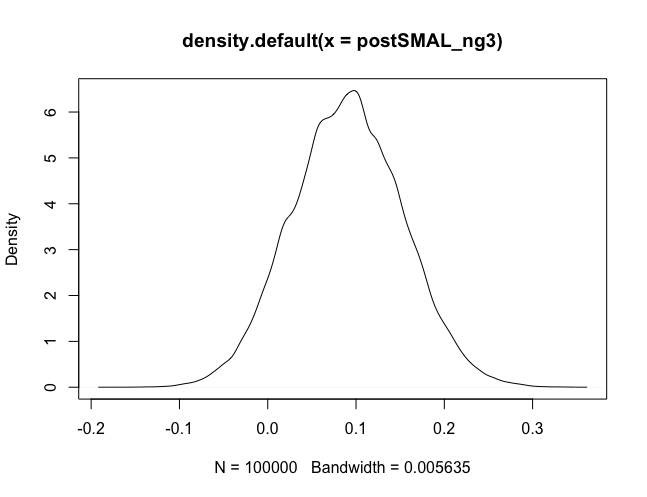
\includegraphics[width=\linewidth]{postSMALng3.png}  
  \label{fig:sub-third}
\end{subfigure}
\begin{subfigure}{.32\textwidth}
  \centering
  % include fourth image
  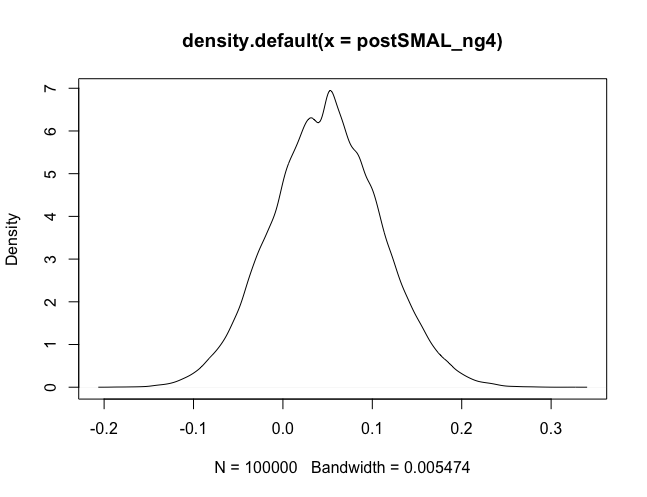
\includegraphics[width=\linewidth]{postSMALng4.png}  
  \label{fig:sub-fourth}
\end{subfigure}
\caption{Posterior distributions of Spearman's $\rho$ for the opposite correlation.}
\label{fig:fig}
\end{figure}
From the density plot we can tell the curve shifts to the right when adding the correlation from $-1$ to $1$ for the equal correlation case, and from the opposite correlation case, the curve keeps shifting to the right when $a$ is decreasing. To see this in a clearer way, we saved the mean of the posterior distributions of the SMAL distributions from those two cases.
\begin{table}[]
\centering
\begin{tabular}{|c|c|c|c|c|}
\hline
\multicolumn{5}{|c|}{Spearman's rho for equal correlation}              \\ \hline
(1,-1,-1,1) & (1,-0.5,-0.5,1) & (1,0,0,1) & (1,0.5,0.5,1)  & (1,1,1,1)  \\ \hline
0.029021    & 0.079083        & 0.1338221 & 0.186915       & 0.248423   \\ \hline
\multicolumn{5}{|c|}{Spearman's rho for opposite correlation}           \\ \hline
(1,-1,1,1)  & (1,-0.5,0.5,1)  & (1,0,0,1) & (1,0.5,-0.5,1) & (1,1,-1,1) \\ \hline
0.0487604   & 0.089154        & 0.1338221 & 0.1710109      & 0.2062635  \\ \hline
\end{tabular}
\caption{Simulation study on the Spearman's $\rho$ }
\label{tab:my-table}
\end{table}
The table presents the results as what we mentioned before.

\newpage

\section{Simulation study on tail dependence coefficients}
Now we move to the simulation on the tail dependence coefficients, we give the density plots of the upper and lower tail dependence and the mean of the posterior distributions.

\begin{table}[H]
\centering
\begin{tabular}{|c|c|c|c|c|}
\hline
\multicolumn{5}{|c|}{Upper tail dependence for equal correlation}        \\ \hline
(1,-1,-1,1) & (1,-0.5,-0.5,1) & (1,0,0,1)  & (1,0.5,0.5,1)  & (1,1,1,1)  \\ \hline
0.06604293  & 0.06424079      & 0.06252416 & 0.09316917     & 0.1204435  \\ \hline
\multicolumn{5}{|c|}{Upper tail dependence for opposite correlation}     \\ \hline
(1,-1,1,1)  & (1,-0.5,0.5,1)  & (1,0,0,1)  & (1,0.5,-0.5,1) & (1,1,-1,1) \\ \hline
0.06321448  & 0.06508844      & 0.06252416 & 0.06316775     & 0.09244834 \\ \hline
\end{tabular}
\caption{Simulation study on the upper tail dependence }
\label{tab:my-table}
\end{table}

\begin{table}[H]
\centering
\begin{tabular}{|c|c|c|c|c|}
\hline
\multicolumn{5}{|c|}{Lower tail dependence for equal correlation}            \\ \hline
(1,-1,-1,1)   & (1,-0.5,-0.5,1) & (1,0,0,1)    & (1,0.5,0.5,1)  & (1,1,1,1)  \\ \hline
-0.0008705791 & 0.001986895     & 0.0004194878 & 0.05808117     & 0.08717094 \\ \hline
\multicolumn{5}{|c|}{Lower tail dependence for opposite correlation}         \\ \hline
(1,-1,1,1)    & (1,-0.5,0.5,1)  & (1,0,0,1)    & (1,0.5,-0.5,1) & (1,1,-1,1) \\ \hline
0.000683531   & -0.0007985829   & 0.0004194878 & -7.758008e-05  & 0.08691091 \\ \hline
\end{tabular}
\caption{Simulation study on the lower tail dependence }
\label{tab:my-table}
\end{table}
\begin{figure}[h]
\begin{center}$
\begin{array}{lll}
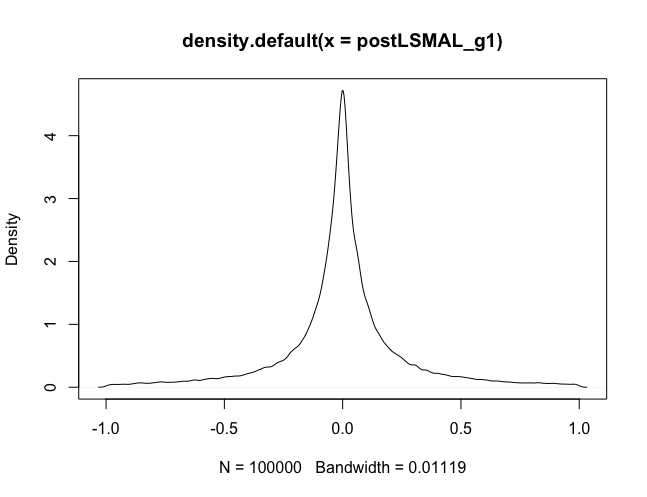
\includegraphics[width=50mm, height=35mm]{postLSMALg1.png}&
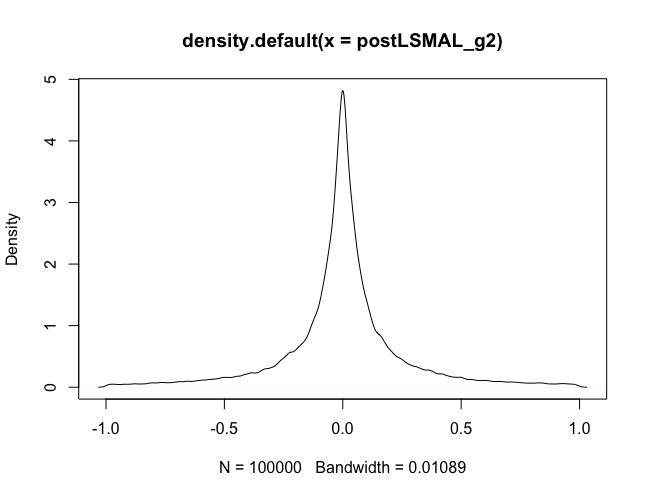
\includegraphics[width=50mm, height=35mm]{postLSMALg2.png}&
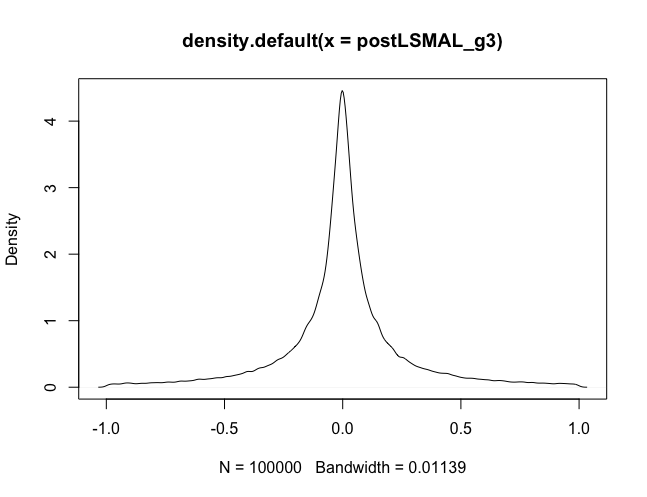
\includegraphics[width=50mm, height=35mm]{postLSMALg3.png}
\end{array}$
\end{center}

\begin{center}$
\begin{array}{rr}
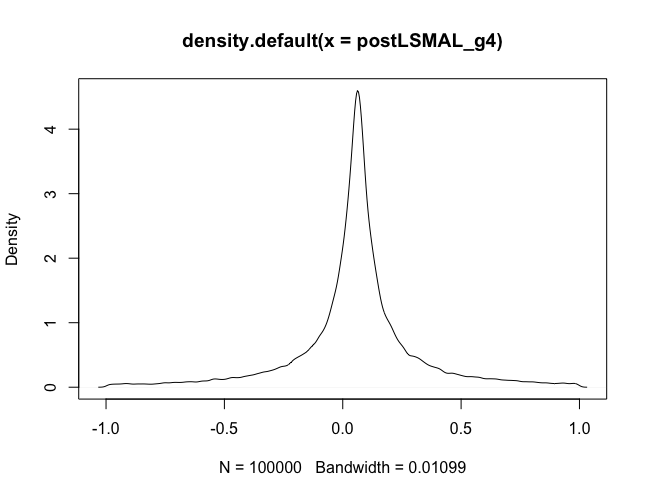
\includegraphics[width=50mm, height=35mm]{postLSMALg4.png}&
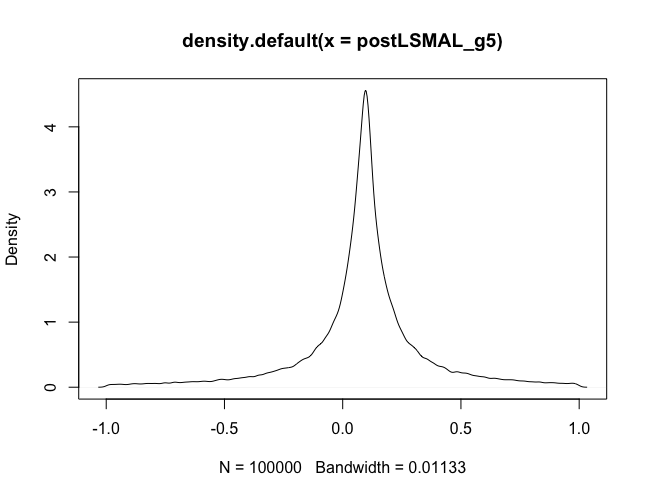
\includegraphics[width=50mm, height=35mm]{postLSMALg5.png}
\end{array}$
\end{center}
\caption{Posterior distributions of $\lambda_L$ for the equal correlation.}
\label{pics:blablabla}
\end{figure}
\newpage
\begin{figure}[h]
\centering
\begin{subfigure}{.32\textwidth}
  \centering
  % include first image
  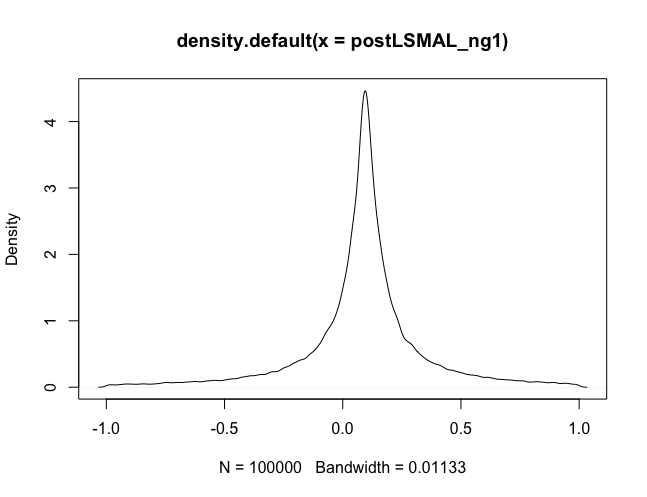
\includegraphics[width=\linewidth]{postLSMALng1.png}  
  \label{fig:sub-first}
\end{subfigure}
\begin{subfigure}{.32\textwidth}
  \centering
  % include second image
  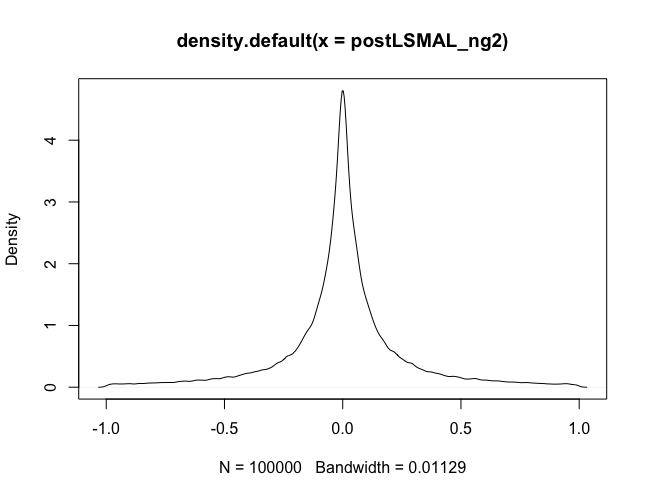
\includegraphics[width=\linewidth]{postLSMALng2.png}  
  \label{fig:sub-second}
\end{subfigure}

\begin{subfigure}{.32\textwidth}
  \centering
  % include third image
  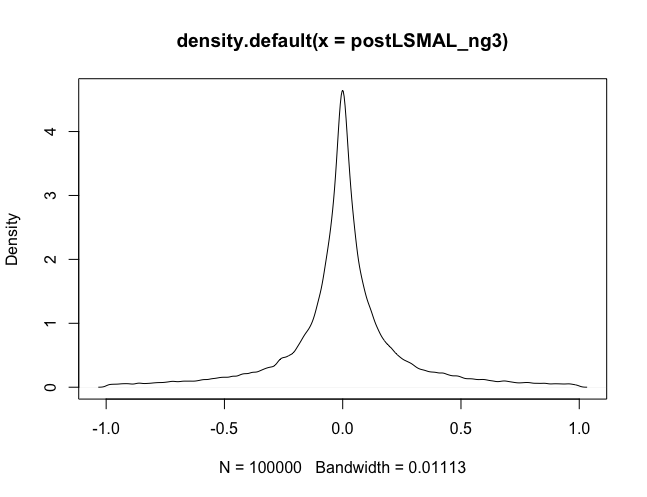
\includegraphics[width=\linewidth]{postLSMALng3.png}  
  \label{fig:sub-third}
\end{subfigure}
\begin{subfigure}{.32\textwidth}
  \centering
  % include fourth image
  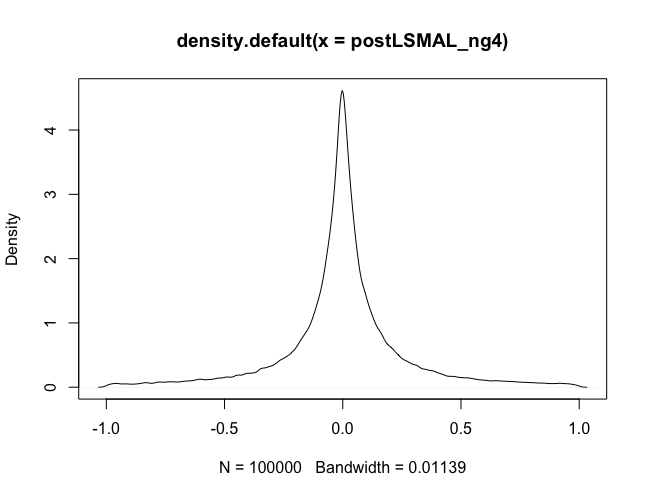
\includegraphics[width=\linewidth]{postLSMALng4.png}  
  \label{fig:sub-fourth}
\end{subfigure}
\caption{Posterior distributions of $\lambda_L$ for the opposite correlation.}
\label{fig:fig}
\end{figure}


\begin{figure}[H]
\begin{center}$
\begin{array}{lll}
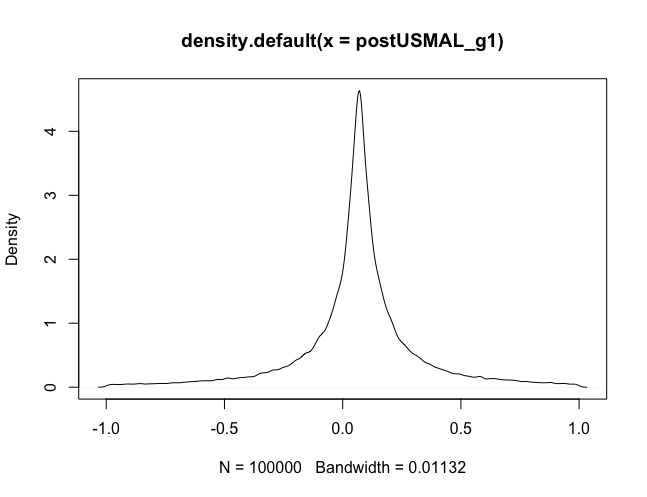
\includegraphics[width=50mm, height=35mm]{postUSMALg1.png}&
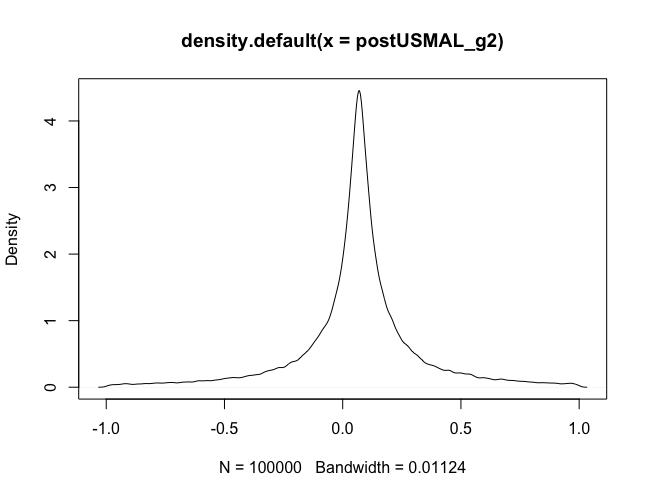
\includegraphics[width=50mm, height=35mm]{postUSMALg2.png}&
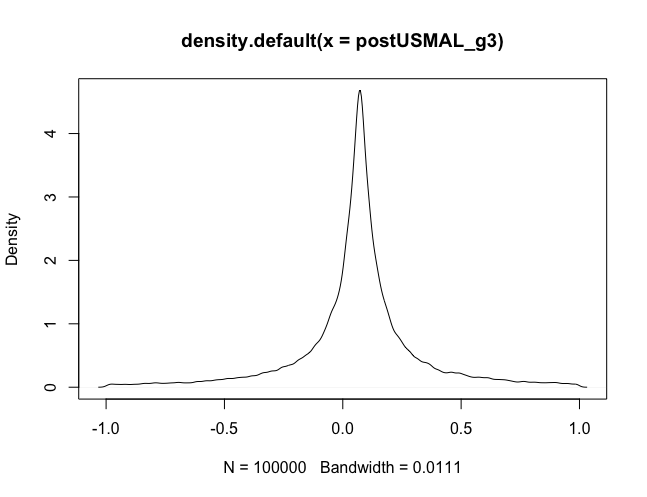
\includegraphics[width=50mm, height=35mm]{postUSMALg3.png}
\end{array}$
\end{center}

\begin{center}$
\begin{array}{rr}
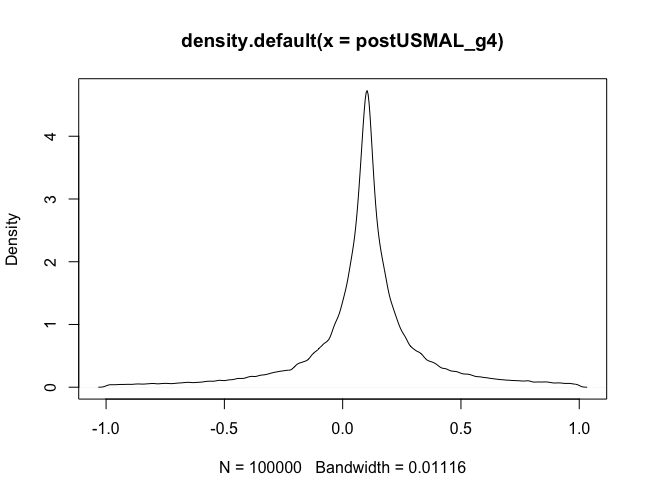
\includegraphics[width=50mm, height=35mm]{postUSMALg4.png}&
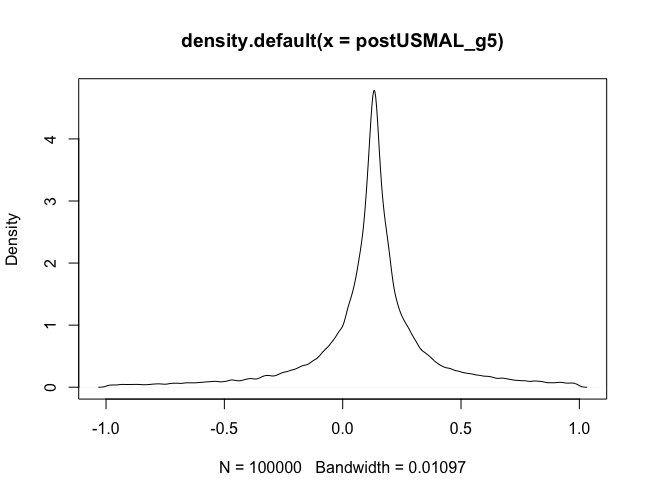
\includegraphics[width=50mm, height=35mm]{postUSMALg5.png}
\end{array}$
\end{center}
\caption{Posterior distributions of $\lambda_U$ for the equal correlation.}
\label{pics:blablabla}
\end{figure}
\begin{figure}[h]
\centering
\begin{subfigure}{.32\textwidth}
  \centering
  % include first image
  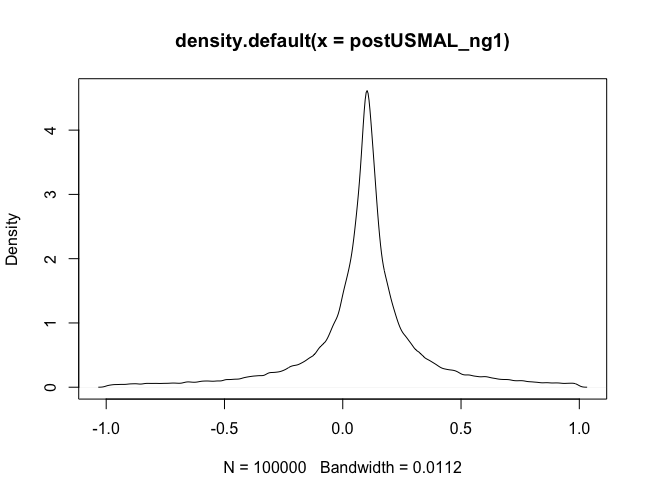
\includegraphics[width=\linewidth]{postUSMALng1.png}  
  \label{fig:sub-first}
\end{subfigure}
\begin{subfigure}{.32\textwidth}
  \centering
  % include second image
  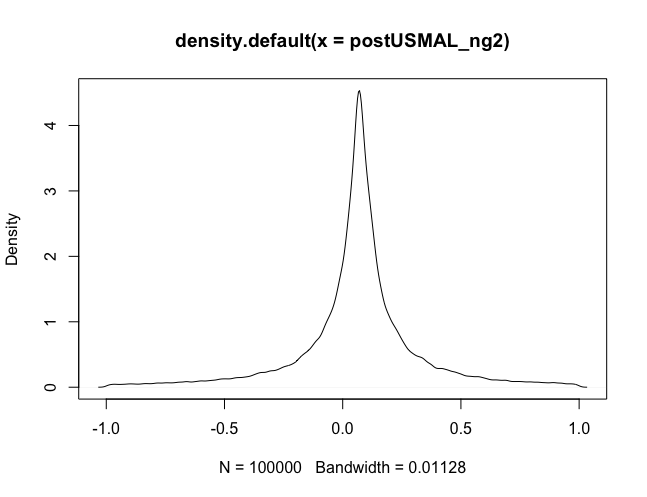
\includegraphics[width=\linewidth]{postUSMALng2.png}  
  \label{fig:sub-second}
\end{subfigure}

\begin{subfigure}{.32\textwidth}
  \centering
  % include third image
  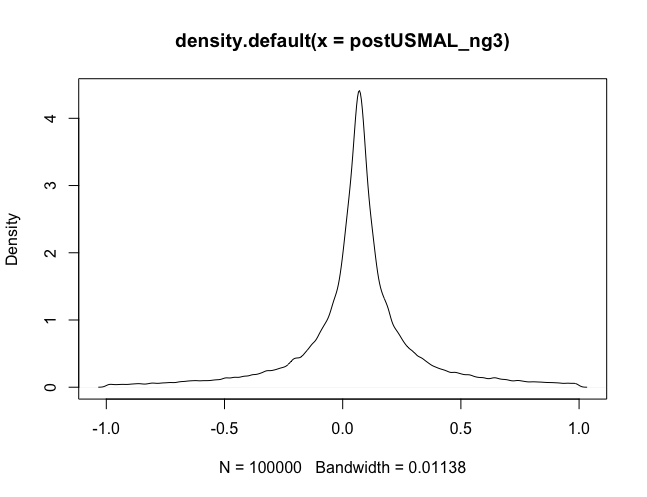
\includegraphics[width=\linewidth]{postUSMALng3.png}  
  \label{fig:sub-third}
\end{subfigure}
\begin{subfigure}{.32\textwidth}
  \centering
  % include fourth image
  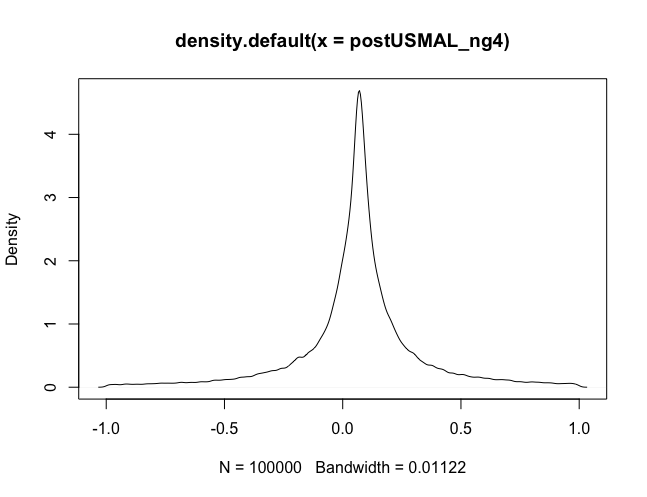
\includegraphics[width=\linewidth]{postUSMALng4.png}  
  \label{fig:sub-fourth}
\end{subfigure}
\caption{Posterior distributions of $\lambda_U$ for the opposite correlation.}
\label{fig:fig}
\end{figure}
By inspecting the means of the posterior distributions and the density plots, we can reach a conclusion that for the upper and lower tail dependence coefficients, the upper and lower tail dependence coefficients barely vary and concentrate around with the change of the correlation matrix.
\newpage




%%%%%%%%%%%%%%%%%%%%%%%%%%%%%%%%%%%%%%%%%%%%%%%%%%%%%%%%%%%%%%%%%%%%
\chapter{Real data inspection}\label{ccl}
%%%%%%%%%%%%%%%%%%%%%%%%%%%%%%%%%%%%%%%%%%%%%%%%%%%%%%%%%%%%%%%%%%%%
Now we want to see if the SMAL distribution fits the real data even if it is very used in practice.
\section{Introduction to the dataset "body"}
The real dataset we will use in our thesis to perform the test is "body" from the R package "gclus". This dataset contains 25 variables, including 21 body dimension measurements along with 4 factors, age, weight, height, and gender. The dataset contains the measurements on 507 individuals. The physical measurements include the chest diameter at nipple level(ChestD), wrist diameter(WristD), chest girth(ChestG), calf maximum girth(CalfG), etc in the unit of centimeter. At first we can take a look at the association between some of the random variables in the dataset.
\begin{figure}[H]
    \centering
    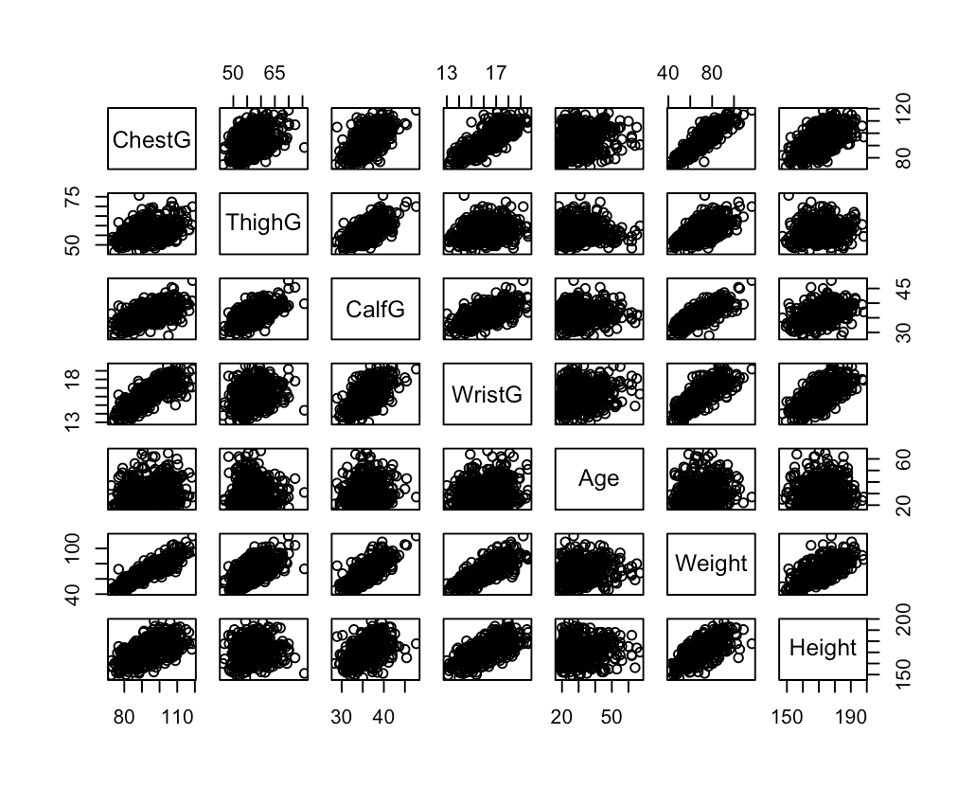
\includegraphics[width=\linewidth]{body.png}
    \caption{Pairs plot of some variables from "body"}
    \label{fig:my_label}
\end{figure}
From the pairs plot, we can conclude that by looking at the first row of the plots, this 
single plot gives us an idea of the relationship between each pair of variables in our dataset. Taking the chest girth(ChestG) as an example, we can tell that this measurement seems to be positive correlated to the weight, and less correlated with age.
\section{Non-parametric Bayesian quantile regression}
We determine to use the calf maximum girth and the thigh maximum girth as two response variables, i.e., $Y=($ Calf maximum girth, Thigh maximum girth $)$ and $X=$(weight, age, BMI index, height), where BMI index = $\matbox{weight}/\matbox{height}^2$ to find the posterior distribution of the Spearman's $\rho$ and the tail dependence coefficients by applying the bivariate analysis by using the Bayesian quantile regression. After applying the algorithm, we can find the results of the non-parametric Bayesian quantile regression on the true dataset. We made the density plots of the Spearman's $\rho$ and the tail dependence coefficients of the true dataset. 
\begin{figure}[H]
\centering
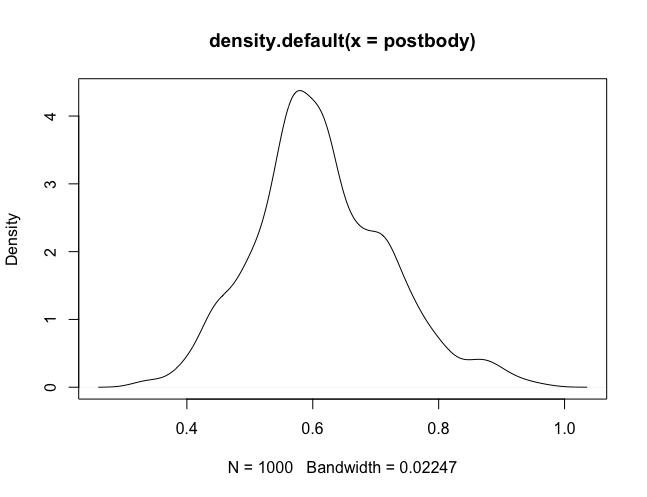
\includegraphics[width=0.5\textwidth,height=0.4\textwidth]{postbody.png}
\caption{Density plot of the posterior distribution of the Spearman's $\rho$ of the real dataset}
\end{figure}

\begin{figure}[H]
\centering
\begin{subfigure}{.42\textwidth}
  \centering
  % include first image
  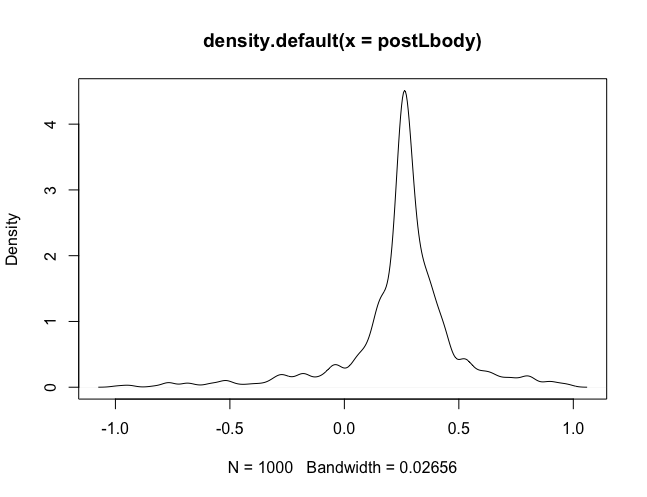
\includegraphics[width=\linewidth]{postLbody.png}  
  \caption{Density plot of the posterior distribution of lower tail dependence coefficient of the real dataset}
  \label{fig:sub-first}
\end{subfigure}
\begin{subfigure}{.42\textwidth}
  \centering
  % include second image
  \includegraphics[width=\linewidth]{postUbody.png}  
  \caption{Density plot of the posterior distribution of upper tail dependence coefficient of the real dataset}
  \label{fig:sub-second}
\end{subfigure}
\caption{density plots of the posterior distributions of the tail dependence coefficients of the real data}
\end{figure}
The above figures gives us the Spearman's $\rho$ concentrates around 0.6 and both the upper and lower tail dependence coefficients for the real data are around 0.3. Since we have a Spearman's $\rho$ at 0.6 which gives a decent correlation between $X$ and $Y$, this means $Y$ can almost be interpreted as a monotone function of $X$. And from the tail dependence coefficients we can tell that the real data sometimes contains the events with the extreme value.
\section{Simulate An SMAL distribution for testing}
In order to test if the SMAL distribution fits the real dataset, we will simulate a new SMAL for testing with the number of dimensions $p=2$, and the number of regressors $k=4$. we set the other parameter fixed as before and then we obtain the following density plots
\begin{figure}[H]
\centering
\includegraphics[width=0.5\textwidth,height=0.4\textwidth]{postSMALtest.png}
\caption{Density plot of the posterior distribution of the Spearman's $\rho$ of the testing SMAL}
\end{figure}

\begin{figure}[H]
\centering
\begin{subfigure}{.42\textwidth}
  \centering
  % include first image
  \includegraphics[width=\linewidth]{postLSMALtest.png}  
  \caption{Density plot of the posterior distribution of lower tail dependence coefficient of the testing SMAL}
  \label{fig:sub-first}
\end{subfigure}
\begin{subfigure}{.42\textwidth}
  \centering
  % include second image
  \includegraphics[width=\linewidth]{postUSMALtest.png}  
  \caption{Density plot of the posterior distribution of upper tail dependence coefficient of the testing SMAL}
  \label{fig:sub-second}
\end{subfigure}
\caption{Density plots of the posterior distributions of the tail dependence coefficients of the testing SMAL}
\end{figure}
\newpage
From the figures above, we will reach a conclusion that both the Spearman's $\rho$ and the tail dependence coefficients are not the same, the Spearman's $\rho$ is about 0.6 in the real dataset instead of 0.2 from the SMAL distribution, also, both of the upper and lower tail dependence coefficients for the real data are around 0.3 instead of 0 from the SMAL.
%%%%%%%%%%%%%%%%%%%%%%%%%%%%%%%%%%%%%%%%%%%%%%%%%%%%%%%%%%%%%%%%%%%%
\chapter{Conclusion}\label{ccl}
In this work, we first introduce the asymmetric Laplace distribution and the multivariate asymmetric Laplace distribution. And we proposed the main point of the thesis : is the dependence structure imposed by the SMAL reasonable for the dataset at hand? To obtain the final result, we introduce the non-parametric Bayesian quantile regression and the most important tool we are using in thesis, copulas. According to the definitions and properties of those commonly used copulas, we implement the Bayesian quantile regression algorithm to test the association between two random variables. And the coefficients we focus on are the Spearman's $\rho$ and the tail dependence coefficients. Spearman's $\rho$ can be used to estimate the correlation between two random variables $X$ and $Y$ and the correlation between these two random variables can be expressed by an monotonic function, when one of the variables can be expressed as a good monotone function of the other variable (i.e., the two variables have the same change trend), the Spearman's $\rho$ between the two variables can reach $+1$ or $-1$. And tail dependence coefficient can be used to estimate the dataset with the extreme value. Also we have conducted the simulation study to find the relationship between the correlation matrix and the dependence structure. Then we apply the test on the real data and make a comparison between the real dataset and the simulating SMAL in the same dimensions and with equal regressors. At last we reach a conclusion that although the SMAL is used for practical reasons, it does not fit our true dataset well. The reason why the SMAL is widely used is just because it has a definition directly on the quantiles, and the
likelihood based on the SMAL can provide an automatic choice of the optimal level of penalization.\\
Of course, there are still some problems to be solved in this thesis and we have the future research prospects, mainly in the following:\\
First of all, we mainly focused on the two-dimensional case. Although bivariate is the basis of multivariate and has the advantages of intuitive and easy to understand, however, how to promote duality to pluralism is still a problem. Especially, when the dimension increases, the complexity of the model and the difficulty of estimation will increase exponentially. There may be other simpler methods to solve these problems. In addition, extreme value theory is also a method developed in recent years to study the extreme value and tail dependence. The combination of copula and tail dependence coefficients can be dig deeper.
%%%%%%%%%%%%%%%%%%%%%%%%%%%%%%%%%%%%%%%%%%%%%%%%%%%%%%%%%%%%%%%%%%%%
%%%%%%%%%%%%%%%%%%%%%%%%%%%%%%%%%%%%%%%%%%%%%%%%%%%%%%%%%%%%%%%%%%%%%%%%%%

\clearpage
\addcontentsline{toc}{chapter}{References}
\bibliographystyle{unswthesis}

\begin{thebibliography}{999}

\bibitem
{GB} Geraci M, Bottai M. Quantile regression for longitudinal data using the asymmetric Laplace distribution. Biostatistics. 2007 Jan;8(1):140-54. doi: 10.1093/biostatistics/kxj039. Epub 2006 Apr 24. PMID: 16636139.

\bibitem
{KK} Kotz, S., Kozubowski, T. J., &amp; Podgórski, K. (2001). The Laplace distribution and generalizations: A revisit with applications to communications, economics, engineering, and finance. New York: Springer.

\bibitem
{LV} Lea Petrella, Valentina Raponi, 2019
Joint estimation of conditional quantiles in multivariate linear regression models with an application to financial distress,
Journal of Multivariate Analysis, Volume 173, Pages 70-84,
ISSN 0047-259X

\bibitem
{C} Christopher M. Bishop (2006). Pattern Recognition and Machine Learning. Springer. pp. 21–24. ISBN 978-0-387-31073-2.

\bibitem
{KB} Koenker, R., & Bassett, G. (1978). Regression Quantiles. Econometrica, 46(1), 33-50. doi:10.2307/1913643

\bibitem
{S}  Martin Haugh (2016). An Introduction to Copulas

\bibitem
{S} Schmidt, T. (2006). Coping with Copulas.

\bibitem
{N}Nelsen, R.B. 2006. An Introduction To Copulas. 2nd ed. Portland.

\bibitem
{C}  Clayton, David G. (1978). "A model for association in bivariate life tables and its application in epidemiological studies of familial tendency in chronic disease incidence". Biometrika. 65 (1): 141–151. doi:10.1093/biomet/65.1.141. JSTOR 2335289.

\bibitem
{GL}Grazian, Clara; Liseo, Brunero. Approximate Bayesian Inference in Semiparametric Copula Models. Bayesian Anal. 12 (2017), no. 4, 991--1016. doi:10.1214/17-BA1080.

\bibitem
{J} Joe, H.(2015). Dependence modeling with copulas, volume 134 of Monographs on Statistics
and Applied Probability. CRC Press, Boca Raton, FL.

\bibitem
{SW}Schweizer, B.; Wolff, E. F. On Nonparametric Measures of Dependence for Random Variables. Ann. Statist. 9 (1981), no. 4, 879--885. doi:10.1214/aos/1176345528. 



\bibitem
{B} Borkowf, C. B. (2002). “Computing the nonnull asymptotic variance and the asymptotic
relative efficiency of Spearman’s rank correlation.” Comput. Statist. Data Anal.,
39(3): 271–286.

\bibitem
{GC} Hartmann, Philip; Straetmans, Stefan T.M.; De Vries, Casper G. (2004). "Asset Market Linkages in Crisis Periods". Review of Economics and Statistics. 86 (1): 313–326. doi:10.1162/003465304323023831.

\bibitem
{S} Sibuya, M. Bivariate extreme statistics, I. Ann Inst Stat Math 11, 195–210 (1960).

\bibitem
{AK} Ane, Thierry;Kharoubi, Cécile. (2003). Dependence Structure and Risk Measure. The Journal of Business. 76. 411-438. 10.1086/375253. 

\bibitem
{HW} Frahm, G., Junker, M., and Schmidt, R. (2005). “Estimating the tail-dependence coefficient:
properties and pitfalls.” Insurance Math. Econom., 37(1): 80–100.

\bibitem
{JS} Joe, H., Smith, R. L., and Weissman, I. (1992). “Bivariate threshold methods for extremes.”
J. Roy. Statist. Soc. Ser. B, 54(1): 171–183.


\bibitem
{SN}Salazar, Y. and Ng, W. L. (2015). “Nonparametric estimation of general multivariate
tail dependence and applications to financial time series.” Statistical Methods \& Applications, 24(1): 121–158.





\end{thebibliography}




\end{document}





